\documentclass[a4paper,german]{article}
%Mainly taken from
%https://github.com/gillescastel/university-setup/blob/master/preamble.tex
%but edited for own purposes

%%%%%OWN
%%Own basic packages
\usepackage{mkessler-math}
\usepackage{mkessler-fancythm}
\usepackage{mkessler-operators}

\usepackage{datetime}
\date{{\normalfont Mitschrift}\\{\sc Maximilian Keßler}}

\usepackage{wrapfig}
\usepackage{pgfplots}
\pgfplotsset{compat=1.7}
%%%%%%Preamble from Gilles Castel
% Some basic packages
\usepackage{url}
\usepackage{graphicx}
\usepackage{float}

% for wrapping text around figures
\usepackage{wrapfig}

%%This option is for now commented out, not sure what it does, but causes errors
%\pdfminorversion=7


% Don't indent paragraphs, leave some space between them
\usepackage{parskip}

% Hide page number when page is empty
\usepackage{emptypage}
% Other font I sometimes use.
\usepackage{xcolor}
% \usepackage{cmbright}

% Math stuff
\usepackage{amsfonts}

% Put x \to \infty below \lim
\let\svlim\lim\def\lim{\svlim\limits}

%Make implies and impliedby shorter
\let\implies\Rightarrow
\let\impliedby\Leftarrow
\let\iff\Leftrightarrow
\let\epsilon\varepsilon

% Command for short corrections
% Usage: 1+1=\correct{3}{2}

% Environments
\makeatother

% Fix some spacing
% http://tex.stackexchange.com/questions/22119/how-can-i-change-the-spacing-before-theorems-with-amsthm
\makeatletter
\def\thm@space@setup{%
  \thm@preskip=\parskip \thm@postskip=0pt
}


% \lecture starts a new lecture (les in dutch)
%
% Usage:
% \lecture{1}{di 12 feb 2019 16:00}{Inleiding}
%
% This adds a section heading with the number / title of the lecture and a
% margin paragraph with the date.

% I use \dateparts here to hide the year (2019). This way, I can easily parse
% the date of each lecture unambiguously while still having a human-friendly
% short format printed to the pdf.

\usepackage{xifthen}
\def\testdateparts#1{\dateparts#1\relax}
\def\dateparts#1 #2 #3 #4 #5\relax{
    \marginpar{\small\textsf{\mbox{#1 #2 #3 #5}}}
}

\def\@lecture{}%
\newcommand{\lecture}[3]{
    \ifthenelse{\isempty{#3}}{%
    \def\@lecture{\ifenglish Lecture\else Vorlesung\fi\, #1}%
    }{%
\def\@lecture{\ifenglish Lecture\else Vorlesung\fi\, #1: #3}%
    }%
    \subsection*{\@lecture}
    \marginpar{\small\textsf{\mbox{#2}}}
}

% These are the fancy headers
\usepackage{fancyhdr}
\pagestyle{fancy}

% LE: left even
% RO: right odd
% CE, CO: center even, center odd
% My name for when I print my lecture notes to use for an open book exam.
% \fancyhead[LE,RO]{Gilles Castel}

\fancyhead[RO,LE]{\@lecture} % Right odd,  Left even
\fancyhead[RE,LO]{}          % Right even, Left odd

\fancyfoot[RO,LE]{\thepage}  % Right odd,  Left even
\fancyfoot[RE,LO]{}          % Right even, Left odd
\fancyfoot[C]{\leftmark}     % Center

\makeatother

% Todonotes and inline notes in fancy boxes
\usepackage{todonotes}

% Make boxes breakable
\tcbuselibrary{breakable}

% Figure support as explained in my blog post.
\usepackage{import}
\usepackage{xifthen}
\usepackage{pdfpages}
\usepackage{transparent}
\newcommand{\incfig}[1]{%
    \def\svgwidth{\columnwidth}
    \import{./figures/}{#1.pdf_tex}
}

% Fix some stuff
% %http://tex.stackexchange.com/questions/76273/multiple-pdfs-with-page-group-included-in-a-single-page-warning
\pdfsuppresswarningpagegroup=1






\title{{Einführung in die} \\ Geometrie und Topologie}
\author{{\normalfont Dozent}\\{\sc Dr. Daniel Kasprowski}}

\def\twedge{\vee}
\def\tsmash{\wedge}

\begin{document}
    \maketitle
    \vspace{3em}
    \centering \small Version \\
    \today\; \currenttime
    \vspace{10em}
    \abstract{Bei folgenden Vorlesungsnotizen handelt es sich um (inoffizielle) Mitschriften zur 'Einführung in die Geometrie und Topologie', die im Sommersemester 2021 an der Universität Bonn gehalten wird. Ich garantiere weder für Korrektheit noch Vollständigkeit dieser Notizen, und bin dankbar für jegliche Art von Korrektur, sowohl inhaltlich, als auch Tippfehler. \\
Bemerkungen oder andere Umgebungen, die nicht zum eigentlichen Vorlesungsinhalt gehören, wurden mit einem * gekennzeichnet. Sie werden nach eigenem Ermessen hinzugefügt, um weitere Details oder evtl. mündliche Anmerkungen beizufügen. Insbesondere sind diese wohl besonders fehleranfällig, also verlasst euch nicht auf sie.\\
Manche Umgebungen sind mit einem $^{\dagger}$ versehen. Das ist dann der Fall, wenn ihr Inhalt so, oder zumindest in sehr ähnlicher Form, in der Vorlesung vorkam (unter Umständen auch mündlich), ich aber die Umgebung der Aussage geändert habe. Das ist z.B. dann der Fall, wenn ich aus Aussagen, die einfach erwähnt werden, ein \textbf{Lemma$^{\dagger}$} mache, um sie hervorzuheben. \\
Weitere Informationen finden sich bei \href{https://github.com/kesslermaximilian/LectureNotesBonn}{GitHub} oder auf der \href{http://www.math.uni-bonn.de/people/daniel/2021/geotopo/}{Vorlesungshomepage}.}

    \newpage
    \tableofcontents
    \newpage
    \listoflecture
    \addcontentsline{toc}{section}{Übersicht der Vorlesungen}
    \newpage
    % start lectures
    \lecture{1}{Mo 12 Apr 2021 10:16}{Grundbegriffe}

\begin{itemize}
    \item Es gibt ein Helpdesk, auch explizit für Studentinnen
    \item die Vorlesung wird aufgenommen, und zwar ohne Videos der Teilnehmenden sowie des Dozenten, die Aufzeichnung werden anschließend in Sciebo hochgeladen.
    \item Es gibt ein Diskussionsforum für Fragen (auf eCampus).
    \item Ab heute Abend, 18 Uhr (Mo 12 Apr 2021 18:00), kann man sich auf eCampus für die Übungsgruppen registrieren und endet am Dienstag Abend um 24 Uhr (Di 12 Apr 2021 24:00), es wird versucht, die Studenten gleichmäßig zu verteilen.
    \item Falls ihr in der Warteliste landet und gewünscht ist, in der Gruppe abzugeben, schreibt eine Mail mit den gewünschten Abgabepartner, dann kann eine gemeinse Einteilung erfolgen.
    \item Es gibt auch das Modul \verb?AlmaIIb?. Registriert euch noch nicht, dies ist für den 2. Teil der Vorlesung notwendig. 
    \item Die Abgabe der Übungsblätter erfolgt einheitlich jeden Freitag um 12 Uhr.
    \item Gruppenabgaben sind erlaubt, bis zu einer Größe von maximal 4 StudentInnen.
    \item Das 1. Blatt ist freiwillig und gibt Bonuspunkte.
    \item Für die Klausurzulassung werden 50\% der Punkte benötigt. Von den Programmieraufgaben müssen mindestens 4 von 6 zufriedenstellend bearbeitet werden.
    \item Programmieraufgaben gibt es ab dem 2. Übungsblatt auf jedem 2. Blatt. Die Bearbeitungszeit beträgt dann 2 Wochen.
\end{itemize}


\section*{Einleitung}
In der Vorlesung werden wir sehen:
\begin{description}
    \item[Teil 1: Diskrete Stochastik]
        \begin{itemize}
            \item Zufallsvariablen
            \item Bedingte Wahrscheinlichkeiten
            \item Unabhängigkeit von Variablen
            \item Monte-Carlo Methoden
        \end{itemize}
    \item[Teil 2: Numerische Analysis]
        \begin{itemize}
            \item Iterative Verfahren
            \item Interpolation von Daten (durch Polynome, trigonometrische Funktionen, \ldots)
            \item Numerische Verfahren für die Integration
        \end{itemize}
\end{description}


\section{Diskrete Stochastik}
\subsection{Einleitung}
\begin{goal}
    Beschreibung von Systemen, die einen Anteil an \vocab{Zufall} haben, d.h. nicht 100\% deterministisch sind.
\end{goal}
\begin{example}
    \begin{itemize}
        \item Spiele: Kartenspiele, Glücksspiele, \ldots
        \item Statistik: Umfragen, Versicherung
        \item Komplexe Systeme: Wettermodelle, Finanzmärkte
    \end{itemize}
\end{example}

\underline{Was sind Quellen von Zufall?}
\begin{itemize}
    \item Zu komplexe Systeme. Dann sieht der Gesamteffekt zufällig aus.
    \item Fehlende Informationen (z.B. bei einem Kartenspiel)
    \item Chaotische Systeme (Wetter
    \item Intrinsisch unvorhersagbare Systeme (z.B. radioaktiver Zerfall)
\end{itemize}
\begin{question}
    \begin{enumerate}[(1)]
        \item Wie modelliert man ein System mit Zufall?
        \item Wie simuliert man ein System mit Zufall? (anwendungstechnischer)
        \item Welche Voraussagen kann man machen?
    \end{enumerate}
\end{question}


\begin{example}
    Die \vocab{Brown'sche Bewegung}. Das System ist implizit ein Pollen mit vielen Wassermolekülen ($\sim 10^{23})$, die sich im Prinzip deterministisch bewegen. \\
    $\implies$ Wir erhalten ein Gleichungssystem mit $(N+1)\cdot 6$ (3 Positionen, 3 Geschwindigkeit) Variablen. Dieses ist de facto unlösbar. \\

    Was wollen wir hier eigentlich untersuchen? -> Die Bewegung des Pollens, jedoch nicht die der einzelnen Wassermoleküle. \\
    In einer \vocab{Modellierung} ersetzt man die Stöße, die ,durch die Wassermoleküle entstehen durch \vocab{zufällige Stöße}. 
\end{example}

\underline{Diskretes Modell:} Die Zeit bewegt sich in $n\in \left \{0,1,2,\ldots\right\} $. Sei
\[
    Z(n) := (\text{Position des Pollens zur Zeit $n$}) \in  \Z^3
.\] 
OBdA setzen wir $Z(0) = 0$. \\
\underline{Dynamik}: $Z(n+1) = Z(n) + \xi_n$, wobei wir $\xi_n$ aus dem Ergebnis eines Würfelwurfs bestimmen werden:
 \[
\xi_n = \begin{cases}
    (1,0,0) & \text{wenn Würfel}=1 \\
    (-1,0,0) & \text{wenn Würfel}=2 \\
    (0,1,0) & \text{wenn Würfel}=3 \\
    (0,-1,0) & \text{wenn Würfel}=4 \\
    (0,0,1) & \text{wenn Würfel}=5 \\
    (0,0,-1) & \text{wenn Würfel}=6
\end{cases}
.\] 

\begin{question}
    Welche Fragen können wir mit solch einem System nun beantworten? Was pasiert, wenn $n\gg 1$?
\end{question}
\begin{enumerate}[\protect\circled{\alph*}]
    \item Typischerweise erhalten wir $\abs{Z(n)} =  O(\sqrt{n}) $ 
    \item Wenn wir die Frequenz von $[Z(n)]_i$ betrachten, (d.h. bei welcher Koordinate in Richtung $i$ befinden wir uns nach  $n$ Würfen) sehen wir typischerweise: 
        \begin{figure}[h]
            \centering
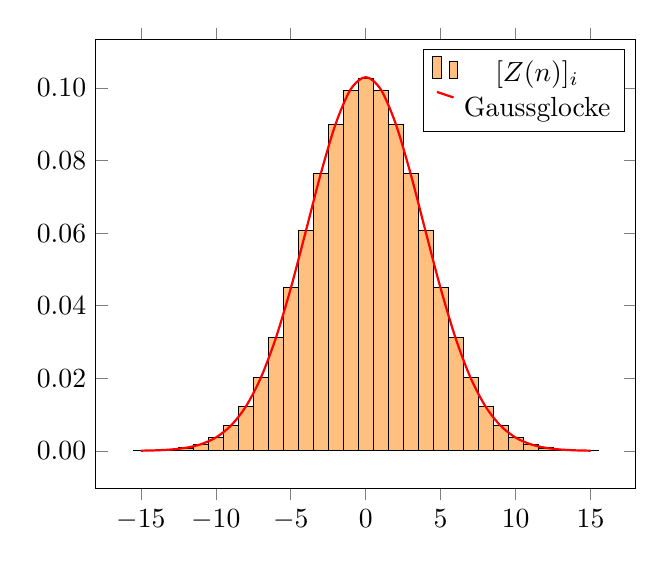
\begin{tikzpicture}[
    declare function={binom(\k,\n,\p)=\n!/(\k!*(\n-\k)!)*\p^\k*(1-\p)^(\n-\k);}
]
\begin{axis}[
    samples at={-15,...,15},
    yticklabel style={
        /pgf/number format/fixed,
        /pgf/number format/fixed zerofill,
        /pgf/number format/precision=2
    },
    ybar=0pt, bar width=1
]
\addplot [fill=orange, fill opacity=0.5] {binom(x+30,60,0.5)}; \addlegendentry{$[Z(n)]_i$}
    \addplot[draw=red,thick,smooth] {1/(sqrt(30*pi)) *exp(-1/30*x^2)}; \addlegendentry{\text{Gaussglocke}}
\end{axis}
\end{tikzpicture}
\caption{Binomialverteilung und Gaussglocke}
\end{figure}
Für $n\gg 1$ sieht diese Verteilung dann ungefähr wie die Gaussglocke aus. \\
\end{enumerate}
\underline{Skalierung:} Wir setzen nun
\[
    B(t) = \lim_{n \to \infty} \frac{Z(\left\lfloor nt \right\rfloor )}{\sqrt{n} }
.\] 
und dies ist dann die Brownsche Bewegung.

Nun möchten wir Vorhersagen treffen können:
\begin{question}
        Ist $Z(n)$ in einer gegebenen Menge  $A$?
\end{question}
Das kann man (im Allgemeinen) nicht einfach mit 'Ja' oder 'Nein' beantworten. Stattdessen müssen wir fragen:
\begin{question}
Wenn man $Z(n)$ beobachtet, wie häufig wird  $Z(n)$ in  $A$ sein?
\end{question}
Diese Frage lässt sich mit einer Zahl $\in [0,1]$ beantworten.

\subsection{Ereignisse und Wahrscheinlichkeiten}
Wir benötigen 3 Grundelemente:
\begin{enumerate}[(1)]
    \item Die Menge $\Omega$ von möglichen \vocab{Ergebnissen}. die Elemente von $\Omega$ heißen auch  \vocab{Elementarereignisse}.
    \item Die Menge $\mathcal{F}$ der \vocab{Ereignisse}. Ein Ereignis  $E$ ist eine Eigenschaft, die mit einer Teilmenge $G\subset \Omega$ assoziiert ist: $ω\in G \iff $ Eigenschaft $E$ ist erfüllt.
    \item Eine \vocab{Wahrscheinlichkeitsverteilung (auch W-maß)}:
        \[
            \mathbb{P}: \mathcal{F} \to  [0,1]
        .\] 
\end{enumerate}
\begin{remark*}
    Wir werden noch sehen, dass gewisse Dinge für unsere Begriffe erfüllt sein müssen, dazu aber später mehr.
\end{remark*}

\begin{example}
    Eine Urne hat 12 nummerierte Kugeln (von 1 bis 12).
    \begin{enumerate}[(1)]
        \item Das \vocab{Zufallsexperiment} besteht daraus, dass wir eine Kugel aus der Urne ziehen und die Zahl notieren, die wir sehen. D.h.
            \[
            \Omega = \left \{1,\ldots,12\right\} 
            .\] 
            Ein Elementarereignis ist nun z.B. gegeben durch $ω = \left \{5\right\}  \equiv 5$ (wir vereinfachen die Notation).
        \item Mögliche Ereignisse sind z.B:
            \begin{equation}
                \begin{split}
                    A &= \text{'Die Zahl ist gerade'} \\
                    B&= \text{'Die Zahl ist }\leq 5 \text{'}\\
                    C &= \text{'Die Zahl ist 8'}
                \end{split}
            \end{equation}
            Die assoziierten Mengen sind dann
            \begin{equation}
                \begin{split}
                    A &= \left \{2,4,6,8,10,12\right\}  \\
                     B &= \left \{1,2,3,4,5\right\} \\
                      C & = \left \{8\right\} 
                \end{split}
            \end{equation}
        \item Für die Wahrscheinlichkeiten nehmen wir an, dass jede Kugel die gleiche Chance hat, gezogen zu werden, d.h.
            \[
                \forall G\in \mathcal{F}: \mathbb{P}(G) = \frac{\abs{G}}{\abs{\Omega} }
            .\] 
            Wir erhalten nun die Wahrscheinlichkeiten
            \[
                \mathbb{P}(A) = \frac{6}{12}=\frac{1}{2} \qquad \mathbb{P}(B) = \frac{5}{12} \qquad \mathbb{P}(C) = \frac{1}{12}
            .\] 
    \end{enumerate}
\end{example}

\begin{notation}
    $A\equiv \left \{ω\in \Omega \mid  ω\in A\right\} \equiv  \left \{ω\in A\right\} \equiv \left \{A \text{ tritt ein}\right\} $
\end{notation}







    %! TEX root = ./master.tex
\lecture[$σ$-Algebren, Messräume. Wahrscheinlichkeitsverteilungen, Wahrscheinlichkeitsräume. Einschluss-Ausschluss-Prinzip. Endliche (diskrete) Wahrscheinlichkeitsräume.]{Mi 14 Apr 2021 10:17}{}
Wir kennen nun die Grundbegriffe $\Omega, \mathcal{F}, \mathbb{P}$ zur Beschreibung von Zufallsexperimenten. Diese wollen wir uns nun genauer ansehen:
\begin{question}
    Welche Struktur muss $\mathcal{F}$ besitzen?
\end{question}
Seien $A,B\in \mathcal{F}$. Dann kann man das Ereignis $A \cap B$ betrachten, also das beide der Eigeschaften eintreten. Genauso sollte
 \[
A^{c} := \Omega \setminus A 
.\] 
, das \vocab{Komplement von $A$}, bzw. das \vocab{Gegenereignis} von $A$ ebenfalls in  $\mathcal{F}$  sein. Aus diesen beiden Eigenschaften folgt bereits, dass
\[
    A \cup B= (A^{c} \cap B^{c})^{c}
.\] 
ebenfalls in $\mathcal{F}$ sein muss. \\
Eine Menge $\mathcal{F}$ mit solchen Eigenschaften heißt \vocab{Algebra}.
\begin{dnotation}
Seien nun $A,B$ und $(A_i)_{i\in I}$  Ereignisse, wobei $I$ endlich oder abzählbar ist. Dann notieren wir die folgenden Ereignisse wie folgt:
\begin{enumerate}[label=\protect\circled{\alph*}]
    \item \emphasize{$A \cup B$} : $ω\in A \cup B \iff  ω\in A \lor ω\in B$, d.h. $A\cup B$ tritt ein, genau dann, wenn  $A$ eintritt oder  $B$ eintritt.
        \item  \emphasize{$\bigcup_{i \in  I} A_i$}: $ω\in \bigcup_{i \in  I} A_i$, wenn es ein $i\in I$ gibt, sodass $\omega \in A_i$ ist.
    \item  \emphasize{$A \cap B$}: $\omega\in A \cap B \iff  $ A \underline{und} B treten ein.
        \item \emphasize{$\bigcap_{i \in I} A_i$}: $\omega\in \bigcap_{i \in I}A_i \iff \forall i \in I \colon$ $A_i$ tritt ein.
            \item \emphasize{$A = \emptyset$} ist das Ereignis, welches  \underline{nie} eintritt. \\
                \emphasize{$A = \Omega$} ist das Ereignis, welches \underline{immer} eintritt.
\end{enumerate}
\end{dnotation}

\begin{definition}[$\sigma$-Algebra]\label{def:sigma-algebra}
    Eine  \vocab{$\sigma$-Algebra} ist eine nicht leere Menge $\mathcal{F}$ von Teilmengen von $\Omega$ mit den Eigenschaften:
    \begin{enumerate}[label=\protect\circled{\alph*}]
        \item $\Omega \in \mathcal{F}$
        \item $\forall A\in \mathcal{F} \colon A^{c}\in \mathcal{F}$.
        \item Falls $(A_i)_{i \in I}\in \mathcal{F}$, dann auch $\bigcup_{i=1} ^{\infty}A_i \in \mathcal{F}$.
    \end{enumerate}
    Wir nennen $(\Omega,\mathcal{F})$ dann einen \vocab{Messraum}. 
\end{definition}

\begin{lemma}\label{lm:weitere-eigenschaften-einer-sigma-algebra}
    Sei $\mathcal{F}$ eine $\sigma$-Algebra, dann gilt:
    \begin{enumerate}[label=\protect\circled{\alph*}]
        \item $\emptyset\in \mathcal{F}$
        \item $A,B \in \mathcal{F} \implies A \cup B \in \mathcal{F}$ und $A\cap B \in \mathcal{F}$.
        \item $(A_i)_{i \in I}\in \mathcal{F} \implies \bigcap_{i=1}^{\infty}A_i \in \mathcal{F}$.
    \end{enumerate}
\end{lemma}
\begin{proof}
    \begin{enumerate}[label=\protect\circled{\alph*}]
        \item $\emptyset = \Omega^{c} \in \mathcal{F}$ nach Eigenschaften \circled{a} und \circled{b} aus der Definition.
        \item $A \cup B = A \cup B \cup \emptyset \cup \emptyset \ldots \in \mathcal{F}$ nach Eigenschaften  \circled{b} und \circled{c}. $A \cap B = (A^{c}\cup B ^{c})^{c} \in \mathcal{F}$
        \item $\bigcap_{i=1}^{\infty}A_i = \left( \bigcup_{i=1}^{\infty}A_i^{c} \right) ^{c}\in \mathcal{F}$ nach \circled{b} und \circled{c}.
    \end{enumerate}
\end{proof}

Wir haben nun $(\Omega, \mathcal{F})$ näher untersucht, es fehlt noch $\mathbb{P}$. 
\begin{question}
    Welche Eigenschaften soll $\mathbb{P}$ (das Wahrscheinlichkeitsmaß bzw. die Wahrscheinlichkeitsverteilung) besitzen?
\end{question}
Seien $A,B \in \mathcal{F}$ mit $A\cap B = \emptyset$, d.h. $A$ und $B$ können nicht gleichzeitig eintreten. Dann fordern wir
\[
    \mathbb{P}(A \cap B) = \mathbb{P}(A) + \mathbb{P}(B) \quad \text{(endliche Additivität)}
.\] 
Dazu soll gelten, dass $\Omega \in \mathcal{F}$ immer eintritt, also $\mathbb{P}(\Omega) = 1 \equiv  100\%$ (Normierung).

\begin{definition}[Wahrscheinlichkeitsverteilung]\label{def:wahrscheinlichkeitsverteilung}
Sei $(\Omega, \mathcal{F})$ ein Messraum. Eine Abbildung $\mathbb{P} : \mathcal{F} \to  \R_+$ ist eine \vocab{Wahrscheinlichkeitsverteilung} auf $(\Omega, \mathcal{F})$, falls
    \begin{enumerate}[(1)]
        \item $\mathbb{P}(\Omega) = 1$
        \item Sind $(A_i)_{i \in I}\in \mathcal{F}$ paarweise disjunkt, so ist:
            \[
                \mathbb{P}\left( \bigcup_{i=1}^{\infty}A_i \right) = \sum_{i=1}^{\infty} \mathbb{P}(A_i) \quad (\sigma\text{-Additivität})
            .\] 
    \end{enumerate}
\end{definition}
\begin{remark*}
    Die Definition macht implizit Gebrauch davon, dass die linke Seite überhaupt definiert ist. Dies folgt jedoch daraus, dass $\mathcal{F}$ eine $\sigma$-Algebra ist.
\end{remark*}

\begin{definition}[Wahrscheinlichkeitsraum]\label{def:wahrscheinlichkeitsraum}
    Ein \vocab{Wahrscheinlichkeitsraum $(\Omega, \mathcal{F},\mathbb{P})$} besteht aus einer Menge $\Omega$, einer  $\sigma$-Algebra $F\subset \mathbb{P}\mathcal{(\Omega)}$ und einem Wahrschenilichkeitsmass $\mathbb{P}$ auf $(\Omega, \mathcal{F})$ 
\end{definition}


\begin{lemma}\label{lm:weitere-eigenschaften-eines-wahrscheinlichkeitsraums}
    Sei $(\Omega, \mathcal{F}, \mathbb{P})$ ein Wahrscheinlichkeitsraum. Dann gilt
\begin{enumerate}[label=\protect\circled{\alph*}]
    \item $\mathbb{P}(\emptyset)=0$ 
    \item $\forall A,B\in \mathcal{F}$ mit $A\cap B = \emptyset$ ist
        \[
            \mathbb{P}(A\cup B ) = \mathbb{P}(A) + \mathbb{P}(B)
        .\] 
    \item      $\forall A,B\in \mathcal{F}$ mit $A\subset B$ ist 
        \begin{equation*}
            \begin{split}
                \mathbb{P}(B) &= \mathbb{P}(A) + \mathbb{P}(B \setminus A)  \\
                \mathbb{P}(A^{c}) &= 1 - \mathbb{P}(A) \\
                \mathbb{P}(A) &\leq  \mathbb{P}(B) \leq  1
            \end{split}
        \end{equation*}
    \item $\forall A,B \in \mathcal{F}$ ist
        \begin{equation*}
            \begin{split}
                \mathbb{P}(A \cup B) &= \mathbb{P}(A) + \mathbb{P}(B) - \mathbb{P}(A\cap B) \\
                                     &\leq  \mathbb{P}(A) + \mathbb{P}(B)
            \end{split}
        \end{equation*}
    \item Wenn $A_n \nearrow A$ ,d.h. $A_1\subset A_2\subset \ldots$ mit $\bigcup_{i =1}^{\infty} A_i = A$ (monotone Konvergenz von Mengen) oder $A_n \searrow A$ (d.h.  $A_1\supset A_2 \supset \ldots$ mit $\bigcap_{i=1}^{\infty} A_i = A $ ), so ist
        \[
            \lim_{n \to \infty} \mathbb{P}(A_n) = \mathbb{P}\left( \lim_{n \to \infty} A_n \right)  = \mathbb{P}(A)
        .\] 
\end{enumerate}
\end{lemma}
\begin{proof}
    \begin{enumerate}[label=\protect\circled{\alph*}]
        \item Wir wissen:
            \[
                1= \mathbb{P}(\Omega) = \mathbb{P}\left( \Omega \cup \emptyset \cup \emptyset \cup \emptyset \ldots  \right)  = \mathbb{P}(\Omega) + \mathbb{P}(\emptyset) + \mathbb{P}(\emptyset) + \ldots
            .\] 
            Das Subtrahieren von $\mathbb{P}(\Omega) =1$ liefert dann $\mathbb{P}(\emptyset) = 0$.
        \item Sei $A \cap B = \emptyset$, dann ist:
            \begin{equation*}
                \begin{split}
                    \mathbb{P}(A\cup B ) &= \mathbb{P}(A \cup B \cup \emptyset \cup \emptyset \cup \ldots) \\
                                         &\stackrel{σ-\text{Additivität}}{=} \mathbb{P}(A) + \mathbb{P}(B) + \mathbb{P}(\emptyset) + \mathbb{P}(\emptyset) + \ldots \\
                                         &= \mathbb{P}(A) + \mathbb{P}(B)
                \end{split}
            \end{equation*}
        \item Sei $A\subset B$. Dann ist $B = A \cup (B \setminus A)$ eine disjunkte Vereinigung, also erhalten wir
            \[
                \mathbb{P}(B) = \mathbb{P}(A) + \underbrace{\mathbb{P}(B \setminus A)}_{\geq 0} \geq  \mathbb{P}(A)
            .\] 
            Mit $B = \Omega$ ergibt sich  $1 = \mathbb{P}(A) + \mathbb{P}(A^{c})$.
        \item Es gilt
            \begin{equation}
                \begin{split}
                    \mathbb{P}(A \cup B) &= \mathbb{P}(A) + \mathbb{P}((A \cup B) \setminus A)  \\
                                         &= \mathbb{P}(A) + \mathbb{P}(B \setminus (A \cap B)) \\
                                         &= \mathbb{P}(A) + \mathbb{P}(B) - \underbrace{\mathbb{P}(A \cap B)}_{\geq 0} \\
                                         &\geq \mathbb{P}(A) + \mathbb{P}(B)
                \end{split}
            \end{equation}
        \item Übung
    \end{enumerate}
\end{proof}
\begin{corollary}[Einschluss-Ausschluss-Prinzip]\label{cor:einschluss-ausschluss-prinzip}
    Seien $A_1,\ldots,A_n \in \mathcal{F}$. Dann gilt
    \[
        \mathbb{P}(A_1 \cup \ldots \cup A_n) = \sum_{k=1}^{n} (-1)^{k-1} \sum_{1\leq i_1<i_2<\ldots<i_k \leq n} \mathbb{P}(A_{i_1} \cap A_{i_2} \cap \ldots \cap A_{i_k})
    .\] 
\end{corollary}
\begin{proof}
    Per Induktion: der Induktionsanfang lautet  $\mathbb{P}(A_1) = \mathbb{P}(A_1)$ und ist offensichtlich wahr. \\
    Die Aussage gelte nun für ein $n\in \N$, damit erhält man
    \begin{equation}
        \begin{split}
            \mathbb{P}\left( \bigcup_{i=1}^{n+1} A_i \right)  &= \mathbb{P}\left( \left(\bigcup_{i=1}^{n}A_i \right) \cup A_{n+1}\right)  \\
                                                              &= \mathbb{P}\left(\bigcup_{i=1}^{n} A_i\right) + \mathbb{P}(A_{n+1}) - \mathbb{P}\left( \left( \bigcup_{i=1}^n A_i \right) \cap A_{n+1} \right)  \\
                                                              &= \mathbb{P}\left( \bigcup_{i=1}^{n} A_i \right)  + \mathbb{P}(A_{n+1}) - \mathbb{P}\left( \bigcup_{i=1}^n \underbrace{(A_i \cap _{A_{n+1}})}_{=: \tilde{A}_i} \right)  \\
                                                              &= \sum_{k=1}^{n} (-1)^{k-1} \sum_{1\leq i<\ldots<i_k \leq n} \mathbb{P}(A_{i_1} \cap \ldots \cap A_{i_k}) + \mathbb{P}(A_{n+1}) \\
                                                              &\qquad -\sum_{k=1}^n (-1)^{k-1} \sum_{1\leq i_1 < \ldots < i_k \leq n} \mathbb{P}(\underbrace{\tilde{A}_{i_1} \cap \ldots \cap \tilde{A}_{i_k}}_{A_{i_1} \cap \ldots \cap A_{i_k} \cap A_{n+1}})
        \end{split}
    \end{equation}
    Andererseits gilt aber auch:
    \begin{alignat*}{5}
           &\quad&  &\sum_{k=1} ^{n+1} (-1)^{k-1} \sum_{1\leq i_1<\ldots<i_k \leq  n+1} \mathbb{P}(A_{i_1} \cap \ldots \cap A_{i_k}) &\quad & \\
           &= & &\sum\limits_{k=1}^{n}(-1)^{k-1} \sum\limits_{1\leq i_1< \ldots < i_k \leq  \color{red} n} \mathbb{P}(A_{i_1} \cap \ldots \cap A_{i_k}) & \quad &\Big\}\text{\parbox{2cm}{Terme mit $i_k\leq n$}} \\
           &+& &\underbrace{\sum_{k=2}^{n+2} (-1)^{k-1} \sum_{1\leq i_1<\ldots<i_{k-1}\leq n} \mathbb{P}(A_i \cap \ldots \cap A_{i_{k-1}} \cap A_{n+1})}_{\stackrel{l := k-1}{=} -\sum\limits_{l=1}^n (-1)^{l-1}\sum\limits_{1\leq i_1<...<i_l\leq n} \mathbb{P}(A_{i_1} \cap \ldots \cap A_{i_l} \cap A_{n+1})}& \quad &\Bigg\}\text{\parbox{2cm}{\small Terme mit $i_k = n+1$ und  $k\geq 2$}}\\
           &+& & \mathbb{P}(A_{n+1}) \qquad& \quad  &\Big\}\text{\parbox{2cm}{\small Terme mit $i_k = n+1$ und  $k=1$}}
    \end{alignat*}
    und damit sieht man, dass die beiden Ausdrücke übereinstimmen, also ist der Induktionsschritt erbracht.
\end{proof}


\subsection{Diskrete Verteilungen}
\begin{itemize}
    \item Sei nun $\Omega$ endlich oder abzählbar.
    \item Falls wir $\mathcal{F}$ nicht explizit angeben, wird $\mathcal{F} = \mathcal{P}(\Omega)$ gewählt, d.h.
        \[
            \operatorname{Card} (\mathcal{P}(\Omega)) \equiv \abs{\mathcal{P}(\Omega)} = 2 ^{ \abs{\Omega}} 
        .\] 
\end{itemize}
\begin{example}[Münzwurf]
    Es sei $\Omega = \left \{K,Z\right\}$, wobei $K$ für Kopf stehe und $Z$ für Zahl. Dann ist
    \[
    \mathcal{F} = \left \{\left \{K\right\} ,\left \{Z\right\} ,\left \{Z,K\right\} ,\emptyset\right\} 
    .\] 
    Sei $p\in [0,1]$ die Wahrscheinlichkeit, dass man Kopf erhält. Da $\mathbb{P}$ für alle Elemente aus $\mathcal{F}$ definiert sein muss, erhalten wir
    \[
        \mathbb{P}(\emptyset) = 0 \qquad \mathbb{P}(K) = p, \qquad \mathbb{P}(Z) = \mathbb{P}(K^{c}) = 1-p \qquad \mathbb{P}(\left \{Z,K\right\} ) = \mathbb{P}(\Omega) = 1
    .\] 
\end{example}
\begin{question}[Charakterisierung von diskreter Wahrscheinlichkeit]
Was müssen wir fordern, damit es $\mathbb{P}$ auf $\mathcal{P}(\Omega)$ gibt?
\end{question}
\begin{example}
    $\Omega = \left \{1,2,\ldots,10\right\}$ würde genügen, da dann $\abs{\mathcal{P}(\Omega)}= 2^{\abs{\Omega} }=2^{10} = 1024 $
    endlich (diskret) wäre.
\end{example}

    \lecture{3}{Di 20 Apr 2021 12:16}{Trennungsaxiome, Kompaktheit}
\begin{proof}
    Betrachte die stetige Abbildung
        \begin{equation*}
        f': \left| \begin{array}{c c l} 
            [0,1] & \longrightarrow & S^1\subset \C \\
        t & \longmapsto &  e^{2\pi it}
        \end{array} \right.
    \end{equation*}
    Wir sehen $f'(0) = f'(1) = 1$, also existiert nach der universellen Eigenschaft ein  $f$, sodass folgendes kommutiert: \\
     \begin{tikzcd}
         \left[ 0,1\right] \ar[two heads]{d}\ar{r}{f'} & S^1 \\
         \left[ 0,1 \right] / (0 \sim 1) \ar[swap,two heads]{ur}{f}
    \end{tikzcd}
    und $f$ stetig ist. Zudem ist  $f$ bijektiv. Es bleibt zu zeigen, dass  $f^{-1}$ stetig ist, das zeigen wir jedoch nicht jetzt (ginge mit viel rechnen), sondern später, wenn wir mehr Technik haben. Anschaulich ist das jedoch klar:
\begin{figure}[ht]
    \centering
    \incfig{intervall-und-kreis-sind-homeomorph}
    \caption{$[0,1] / (0\sim 1)$ und $S^1$ sind homöomorph}
    \label{fig:intervall-und-kreis-sind-homeomorph}
\end{figure}
\end{proof}
\begin{remark}
    Die Abbildung
        \begin{equation*}
        \begin{array}{c c l} 
            [0,1) & \longrightarrow & S^1 \\
        t & \longmapsto &  e^{2\pi it}
        \end{array}
    \end{equation*}
    ist stetig und bijektiv, allerdings kein Homöomorphismus, denn $\left[ 0, \frac{1}{2} \right] \subset [0,1)$ ist offen, aber $f(\left[ 0,\frac{1}{2} \right] ) = \left( f^{-1} \right) ^{-1}\left( \left[ 0,\frac{1}{2} \right]  \right) $ ist nicht offen im Kreis.
\end{remark}
\begin{example}
    \begin{itemize}
        \item Sei $X = [0,1]^2 \subset \R$. Identifiziere nun $(t,0) \sim  (t,1)$ sowie $(0,s) \sim  (1,s)$ für $s,t\in [9,1]$. Dann ist $X / \sim $ der Torus.
        \item Sei $X = [0,1] ^2 \subset \R^2$. Identifizieren wir $(t,0) \sim  (t,1)$ sowie $(0,s) \sim  (1, 1-s)$, so erhalten wir die \vocab{Kleinsche Flasche}. 
        \item Betrachte auf dem $\R^{n+1}\setminus \left \{0\right\} $ die Relation $x \sim  λx$ für $λ>0\in \R$. Dann ist $\R^{n+1} / \sim  \cong S^n$. Zunächst ist nämlich die Abbildung
                \begin{equation*}
                f: \left| \begin{array}{c c l} 
                \R^{n+1}\setminus \left \{0\right\}  & \longrightarrow & S^n \\
                x & \longmapsto &  \frac{x}{\lVert x \rVert _2}
                \end{array} \right.
            \end{equation*}
            stetig und die induzierte Abbildung $\R^{n+1} \setminus \left \{0\right\}  / \sim \to  S^n$ ist bijektiv. Das rechnen wir nach: Seien $x\neq y$ mit $d(x,y) < \delta$, so ist:
            \begin{equation}
                \begin{split}
                    d\left( \frac{x}{\lVert x \rVert },\frac{y}{\lVert y \rVert } \right) &\leq d\left( \frac{x}{\lVert x \rVert },\frac{y}{\lVert x \rVert } \right) + d\left( \frac{y}{\lVert x \rVert },\frac{y}{\lVert y \rVert } \right)  \\
                                                                                          &= \frac{1}{\lVert x \rVert } d(x,y) + \sqrt{\sum \left( \frac{y_i}{\lVert x \rVert }-\frac{y_i}{\lVert y \rVert } \right)^2 }  \\
                                                                                          &= \frac{1}{\lVert x \rVert } d(x,y) + \sqrt{\frac{(\lVert x \rVert -\lVert y \rVert )^2}{\lVert x \rVert \lVert y \rVert }} \lVert y \rVert \\
                                                                                          &< \frac{1}{\lVert x \rVert }\cdot \delta + \frac{\delta}{\lVert x \rVert ^2 + \delta \lVert x \rVert }(\lVert x \rVert +\delta) \to  0
                \end{split}
            \end{equation}
            also ist $f$ stetig. Mit der Inklusion  $ι: S^n \to  \R^{n+1} \setminus \left \{0\right\} $ erhalten wir
            \[
            f \circ  ι = \id_{S^n}
            .\] 
            Übung: Daraus folgt bereits, dass $S^n$ die Quotiententopologie trägt.
        \item Setzen wir erneut $X = \R^{n+1} \setminus \left \{0\right\} $, aber diesmal $x \sim  \lambda x$ für $λ\in \R \setminus  \left \{0\right\} $, so heißt der Quotient
            \[
            X / \sim  =: \R P^n
            .\] 
            der \vocab[Raum!reell projektiv]{reelle projektive Raum}.  Es ist
            \[
                \R P^n \cong S^n / (x \sim -x)
            .\] 
            Dies sehen wir mittels folgendem Diagramm: \\
            \begin{tikzcd}
                \R^{n+1} \setminus \left \{0\right\}  \ar[two heads]{d} \ar[shift left]{r}{f} & S^n \ar[shift left]{l}{ι} \ar[two heads]{d} \\
                \R P^n \ar[dashed, shift left]{r}{\overline{f}} & S^n / (x \sim  - x) \ar[dashed, shift left]{l}{\overline{ι}}
            \end{tikzcd}
            \\
            Die Abbildungen $\overline{ι}$ und $\overline{f}$ sind stetig nach der universellen Eigenschaft und invers zueinander.
        \item Sei $X$ ein topologischer Raum und  $A\subset X$ eine Teilmenge. Definiere die Relation $\sim $ durch $a\sim a'$ für $a,a'\in A$ (bzw. erzeuge eine dadurch). Dann setzen wir
            \[
            X / A := X / \sim 
            .\] 
            Es ergibt sich
            \begin{itemize}
                \item $[0,1] / \left \{0,1\right\} \cong S^1$ 
                \item $[0,1] / [0,1)$ hat zwei Punkte  $[0,1)$ und  $\left \{1\right\} $. Es ist $[0,1) \subset [0,1]$ offen, aber $\left \{1\right\} $ nicht, also handelt es sich um den Sierpinski-Raum.
            \end{itemize}
    \end{itemize}
\end{example}
\begin{remark}
    Quotientenräume von metrischen Räumen sind im Allgemeinen nicht metrisierbar.
\end{remark}

\section{Trennungsaxiome}
\begin{definition}[Hausdorff'sch]\label{def:hausdorff}
    Ein topologischer Raum heißt \vocab{Hausdorff} (oder \vocab[Hausdorff!Hausdorffsch]{Hausdorffsch}), wenn $\forall x,y\in X$ mit $x\neq y$ offene Mengen $U_x, U_y\subset X$ existieren mit $x\in U_x$ und $y\in U_y$, sodass $U_x \cap U_y = \emptyset$. Diese Eigenschaft heißt auch Trennungsaxiom\index{Trennungsaxiom} \vocab[Trennungsaxiom!$T_2$]{$T_2$}. \\
    \begin{minipage}{\textwidth}
    \centering    
\begin{minipage}{0.3\textwidth}
        \centering
        \incfig{hausdroff-raum}
    \end{minipage}
    \end{minipage}
\end{definition}

\begin{theorem}\label{thm:metrisierbarer-raum-ist-hausdorff}
    Ist $X$ metrisierbar, so ist  $X$ Hausdorffsch.
\end{theorem}
\begin{proof}
    Sei $d$ eine Metrik auf  $X$, die die Topologie induziert. Seien  $x,y\in X$ mit $x\neq y$. Setze
    \[
        U_x := U\left( x, \frac{d(x,y)}{2} \right) \qquad U_y = U\left( y, \frac{d(x,y)}{2} \right) 
    .\] 
    Dann ist $U_x \cap U_y = \emptyset$, denn für alle $z\in U_x \cap U_y$ ist
    \[
        d(x,y) \leq  d(x,z) + d(z,y) < \frac{d(x,y)}{2} + \frac{d(x,y)}{2} = d(x,y)
    .\] 
    , was nicht sein kann.
\end{proof}
\begin{example}
    $\R^n$ ist Hausdorffsch.
\end{example}
\begin{theorem}\label{thm:hausdorff-impliziert-t1}
    Ist $X$ Hausdorffsch und  $x\in X$, dann ist $\left \{x\right\} \subset X$ abgeschlossen.
    \label{thm:point-in-hausdorff-space-is-closed}
\end{theorem}
\begin{proof}
    Für $y\neq x$ existiert $U_y$ offen mit  $x\not\in U_y$ und $y\in U_y$. Dann ist
    \[
    X \setminus \left \{x\right\}  = \bigcup_{y\neq x} U_y 
    .\] 
    offen.
\end{proof}
\begin{remark}
    Ein topologischer Raum, für den alle $\left \{x\right\} $ abgeschlossen sind, heißt \vocab[Trennungsaxiom!$T_1$]{$T_1$-Raum}.
\end{remark}

\begin{lemma}\label{lm:teilraum-von-hausdorffraum-ist-hausdorff}
    Sei $X$ Hausdorffsch und $A\subset X$ ein Teilraum. Dann ist auch $A$ Hausdorffsch.
\end{lemma}
\begin{proof}
    Sei $x\neq y\in A$. Dann existieren $U_x, U_y\subset X$ offen mit $x\in U_x$ und $y\in U_y$ sowie $U_x \cap U_y = \emptyset$. Dann sind
    \[
    U_x \cap A \qquad U_y \cap A \subset A
    .\] 
    offen in $A$ und erfüllen die Bedingungen.
\end{proof}


\begin{remark}
    Jeder diskrete Raum ist Hausdorffsch. Ist $X$ endlich und Hausdorffsch, so ist  $X$ diskret.
\end{remark}
\begin{proof}
    Für jedes $y\neq x$ existiert ein $U_x^y$ offen mit  $x\in U_x^y$ und $y\not\in U_x^y$. Dann ist aber
    \[
    \left \{x\right\}  = \bigcap_{y\neq x} U_x^{y}
    .\] 
    offen (da $X$ endlich), also ist $X$ diskret. Die Umkehrung ist offensichtlich.
\end{proof}
\begin{example}
    $S^n \subset \R^{n+1}$ ist Hausdorffsch.
\end{example}

\begin{definition}[Normal]\label{def:normal}
    Ein topologischer Raum heißt \vocab[Topologischer Raum!normal]{normal}, falls
    \begin{itemize}
        \item $X$ ist Hausdorffsch
        \item  $\forall A,B\subset X$ abgeschlossen mit $A \cap B = \emptyset$ existieren $U_A, U_B \subset X$ offen mit $A\subset U_A$, $B\subset U_B$ und $U_A \cap U_B = \emptyset$. Diese Eigenschaft heißt auch Trennungsaxiom \vocab[Trennungsaxiom!$T_4$]{$T_4$}. \\
            \begin{minipage}{\textwidth}
                \centering
                \begin{minipage}{0.3\textwidth}
    \incfig{normaler-raum}
                \end{minipage}
            \end{minipage}
    \end{itemize}
\end{definition}


\begin{remark}
    Manchmal gibt es diese Definition auch ohne Hausdorff'sch.
\end{remark}

\begin{theorem}\label{thm:metrischer-raum-ist-normal}
    Ist $X$ metrisierbar, dann ist  $X$ normal.
\end{theorem}

\begin{proof}
    Übung.
\end{proof}

\begin{definition}[Regulär]\label{def:regulär}
    Ein topologischer Raum $X$ heißt  \vocab[Topologischer Raum!regulär]{regulär}, falls $X$ Hausdorff ist und  $\forall  A \subset X$ abgeschlossen und $x\in X \setminus A$ existieren $U_a, U_{x}$ offen mit $A\subset U_A, x\in U_x$ und $U_A \cap U_x = \emptyset$. (Auch Trennungsaxiom \vocab[Trennungsaxiom!$T_3$]{$T_3$} genannt).
\end{definition}

Klar: $T_4 \implies T_3$


\section{Kompaktheit}
Aus der Analysis ist (vielleicht) folgender Satz bekannt.
\begin{theorem}[Heine-Borel]\label{thm:heine-borel}
    Für $X\subset \R^n$ sind äquivalent:
    \begin{enumerate}[1)]
        \item $X$ ist abgeschlossen und beschränkt.
        \item Jede offene Überdeckung von $X$ hat eine endliche Teilüberdeckung
    \end{enumerate}
\end{theorem}

\begin{recap}
    'Jede offene Überdeckung besitzt eine endliche Teilüberdeckung' bedeutet: \\
    Für jede Familie $\left \{U_i\right\} _{i \in I}$ mit $U_i \subset X$ offen und $X \subset \bigcup_{i \in I}U_i$ existiert eine endliche Teilmenge $J\subset I$ mit $X \subset \bigcup_{j\in J} U_j$
\end{recap}
\begin{proof}
    später.
\end{proof}

\begin{definition}[Kompaktheit]\label{def:kompakt}
    Ein topologischer Raum $X$ heißt  \vocab[Topologischer Raum!kompakt]{kompakt}, falls jede offene Überdeckung eine endliche Teilüberdeckung besitzt.
\end{definition}
\begin{remark}
    Manchmal heißt obige Definition auch quasi-kompakt, und kompakt bedeutet dann quasi-kompakt + Hausdorff.
\end{remark}

\begin{example}
   Die Räume
   \[
       [0,1] \subset \R \qquad S^n \subset \R^{n+1}
   .\] 
   sind beide kompakt (nach \ref{thm:heine-borel})
\end{example}

    \lecture{4}{Do 22 Apr 2021 10:15}{}
\begin{example}
    Zur Frage von letzter Woche (wenn wir einen Hausdorff-Raum haben und eine Äquivalenzrelation, deren Klassen abgeschlossen sind, ist dann der Quotient wieder  Hausdorff?): Wähle auf $[0,1]$ die Relation erzeugt von
     \[
    \frac{1}{n} \sim  1 - \frac{1}{n}
    .\] 
    für alle $n\in \N_>0$. Betrachte dann die Abbildung: 
    \[
        [0,1] \twoheadrightarrow [0,1] / \sim 
    .\] 
    Punkturbilder sind endlich, also abgeschlossen. Aber der Raum $[0,1] / \sim $ ist nicht hausdorffsch, denn wri können die Punkte $0,1$ nicht trennen.
\end{example}
\begin{theorem}
    Sei $X$ ein kompakter Raum und  $Y\subset X$ abgeschlossen. Dann ist $Y$ kompakt.
    \label{thm:closed-subset-of-compact-space-is-compact}
\end{theorem}
\begin{proof}
    Sei $\left \{U_i\right\} _{i \in I}$ eine offene Überdeckung von $Y$. Dann existieren $U_i' \subset X$ offen mit $U_i = U_i' \cap Y$. Die Familie
     \[
    \left \{U_i'\right\} _{i \in I}\cup \left \{\underbrace{X \setminus Y}_{\text{offen}}\right\} 
    .\] 
    ist nun eine offene Überdeckung von $X$. Dann existiert $J\subset I$ endlich, so dass
    \[
    \left \{U_j'\right\} _{j\in J} \cup \left \{X \setminus Y\right\} 
    .\] 
    die Menge $X$ überdeckt. Also ist  
    \[
        \left \{\underbrace{U_j' \cap Y}_{U_j}\right\} _{j\in J} \cup \left \{\underbrace{X \setminus Y \cap Y}_{=\emptyset}\right\}  
    \]
    eine endliche Überdeckung für $Y$.
\end{proof}
\begin{theorem}
    Sei $X$ ein Hausdorff-Raum und  $Y\subset X$ kompakt. Dann ist $Y$ abgeschlossen.
    \label{thm:compact-subset-of-hausdorff-space-is-closed}
\end{theorem}

\begin{corollary}
    Ist $X$ kompakt und Hausdorffsch, dann sind äquivalent:
    \label{thm:compact-iff-closed}
\begin{enumerate}[1)]
        \item $Y\subset X$ ist abgeschlossen
        \item $Y$ ist kompakt.
    \end{enumerate}
\end{corollary}
\begin{lemma}
    Sei $X$ ein Hausdorff Raum und  $Y\subset X$ kompakt. Dann existiert $\forall x\in X\setminus Y$ offene Teilmengen $U_{x,Y}$ und $V_{x,Y}$ von $X$ so dass:  $x\in U_{x,Y}$ und $Y\subset V_{x,Y}$ und $U_{x,Y} \cap V_{x,Y} = \emptyset$.
    \label{lm:compact-set-in-hausdorff-space-is-closed}
\end{lemma}
\begin{proof}
    Sei $x\in X\setminus Y$. $\forall y\in Y$ existieren $U_{x,y}$ und $V_{x,y}$ offen mit $x\in U_{x,y}$ und $y\in V_{x,y}$, weil $X$ Hausdorffsch. \\
    Dann ist  $\left \{V_{x,y} \cap Y\right\} _{y\in Y}$ eine offene Überdeckung von $Y$. Also existiert endliche Teilüberdeckung (da  $Y$ kompakt) induziert durch Punkte  $y_1,\ldots,y_n$. Also:
    \[
    Y\subset \bigcup_{i=1}^n V_{x,y_i}
    .\] 
    Sei
    \[
    V_{x,Y} := \bigcup_{i=1}^n V_{x,y_i} \qquad U_{x,Y} := \bigcap_{i=1}^n U_{x,y_i} 
    .\] 
    Es ist auch $x\in U_{x,Y}$, weil $x\in U_{x,y_i}$ für jedes $i$. Wir müssen also noch Disjunktheit prüfen, es ist:
     \[
    U_{x,Y} \cap V_{x,y_i} \subset U_{x,y_i} \cap V_{x,y_i} = \emptyset
    .\] 
    Also auch
    \[
        \emptyset=    U_{x,Y} \cap \bigcup_{i=1}^n V_{x,y_i} = U_{x,Y} \cap V_{x,Y}
    .\]
\end{proof}
    \begin{figure}[H]
    \includegraphics[scale=0.4]{figures/Lemma5.5.pdf}
    \caption{Skizze zum Beweis von Lemma \ref{lm:compact-set-in-hausdorff-space-is-closed}}
\end{figure}
\begin{proof}[Beweis von \ref{thm:compact-subset-of-hausdorff-space-is-closed}]
    Nach dem Lemma existieren $\forall x\in X \setminus Y$ ein $U_{x,Y}$ mit $x\in U_{x,Y}$ und $U_{x,Y} \cap Y = \emptyset$. Also ist
    \[
    X \setminus Y = \bigcup_{x\in X \setminus Y} U_{x,Y}
    .\] 
    offen und somit ist $Y$ abgeschlossen.
\end{proof}


\begin{example}['Gegenbeispiel' zu Satz \ref{thm:compact-subset-of-hausdorff-space-is-closed}]
    Sei $G$ die Gerade mit zwei Urpsrüngen: \\
    Betrachte  $\R\cup \left \{0'\right\} $ mit $U$ Umgebung von  $a\in \R$ falls $\exists ε>0$ mit $(a-ε, a+ε)\subset U$ und $U$ Umgebung von  $0'$ und  $U$ Umgebung von  $0'$, falls  $\exists ε>0$ mit $(-ε,0 \cup (0,ε) \subset U$ und $0' \in U$. \\
    Wir können uns gewissermaßen  $0,0'$ gleichberechtigt vorstellen, nur dass die beiden Punkte verschieden sind. \\
    Dann ist  $[-1,1] \subset G$ kompakt (Übung!), aber nicht abegschlossen, da $0' \in G \setminus [-1,1]$ ist, dies aber keine Umgebung von $0'$ ist.
    \begin{figure}[H]
        \includegraphics[scale=0.4]{figures/line-with-2-origins.pdf}
    \caption{Gerade mit 2 Ursprüngen}
    \end{figure}
\end{example}


\begin{proof}[Beweis von Satz \ref{thm:heine-borel}]
    '$2) \implies 1)$'. Sei $X\subset \R^n$ kompakt. Dann ist sie abgeschlossen nach \ref{thm:compact-subset-of-hausdorff-space-is-closed}. Zudem ist $X\subset \bigcup_{x\in X} U(x,1)$ eine offene Überdeckung. Da $X$ kompakt finden wir endlich viele  $x_1,\ldots,x_n\in X$ mit
    \[
        X \subset \bigcup_{i=1}^n U(x_i,1)
    .\] 
    Also ist
    \[
        \diam(X) \leq  \max \left \{d(x_i,x_j)\right\} +2 < \infty
    .\] 
    und somit ist $X$ auch beschränkt. \\
    ' $1)\implies 2)$'. Da $X$ beschränkt ist,  $\exists m>0$ mit $X\subset [-m,m]^n\subset \R^n$. Da $X$ abgeschlossen ist, genügt es nach \ref{thm:closed-subset-of-compact-space-is-compact} zu zeigen, dass  $[-m,m]^n$ kompakt ist. \\
    Wir führen einen Widerspruchsbeweis, nimm also an, dass  $[-m,m]^n$ nicht kompakt ist. Dann existiert eine offene Überdeckung  $\left \{U_i\right\} _{i \in I}$ ohne endliche Teilüberdeckung. \\
    Unterteile $[-m,m]^n$ in  $2^n$ gleich große Unterwürfel (halbiere jede Seite). Mindestens ein Unterwürfel hat keine endliche Teilüberdeckung. Unterteile diesen Würfel weiter und wähle wieder einen Unterwüfel, der keine endliche Teilüberdeckung hat. \\
    Wir erhalten eine Folge von Würfeln
     \[
         [-m,m]^n =     Q_0 \supset Q_1 \supset Q_2 \supset Q_3 \supset \ldots
    .\] 
    die jeweils keine endliche Teilüberdeckung durch $U_i's$ besitzen. \\
    Sei  $x_i \in Q_i$ beliebig. Dann ist $x_i$ eine Cauchy-Folge, also existiert $x = \lim_{i\to \infty} x_i$, und $x\in Q_0$, da $Q_0$ abgeschlossen. \\
    Somit gibt es ein $U_j$ mit  $x\in U_j$, da die $\left \{U_i\right\} _{i \in I}$ eine Überedeckung von $Q_0$ waren. Damit ist auch $U(x,ε) \subset U_j$ für ein $ε>0$. Wähle einen Würfel $x\in Q_k$ mit Kantenlänge $< \frac{ε}{\sqrt{n} }$, dann ist auch $Q_k \subset U(x,ε) \subset U_j$. Das ist aber ein Widerspruch dazu, dass $Q_k$ keine endliche Teilüberdeckung hat, \contra. \\
    Also ist  $Q_0$ kompakt.
\end{proof}

\begin{theorem}
    Sei $f: X \to  Y$ stetig und surjektiv und $X$ kompakt. Dann ist auch  $Y$ kompakt. 
    \label{thm:image-of-compact-space-is-compact}
\end{theorem}
\begin{proof}
    Sei $\left \{U_i\right\} _{i \in I}$ offene Überdeckung von $Y$. Dann ist
     \[
         \left \{f^{-1}(U_i)\right\} _{i \in I}
    .\] 
    offene Überdeckung von $X$. Da  $X$ kompakt ist, gibt es  $J\subset I$ endlich mit $X = \bigcup_{j\in J} f^{-1}(U_j)$. Dann ist 
    \[
        Y = f(X) = \bigcup_{j\in J} f(f^{-1}(U_j)) = \bigcup_{j\in J} U_j
    .\] 
    Also existiert eine endliche Teilüberdeckung von $Y$.
\end{proof}
\begin{corollary}
    Sei $f: X \to  Y$ stetig, $X$ kompakt und  $Y$ Hausdorff. Dann ist  $f$ abgeschlossen, d.h. $\forall A\subset X$ abgesclhossen ist $f(A) \subset Y$ abgeschlossen.
\end{corollary}
\begin{proof}
    Sei $A\subset X$ abgeschlossen. Dann ist $A$ kompakt. Also ist  $f(A)$ kompakt. Also ist  $f(A)$ abgeschlossen
\end{proof}
\begin{corollary}
    Ist $f: X \to  Y$ stetig und bijektiv, $X$ kompakt und  $Y$ Hausdorff, dann ist  $f$ ein Homöomorphismus.
    \label{cor:compact-to-hausdorff-is-homeomorphism}
\end{corollary}
\begin{proof}
    Wir müssen zeigen, dass die Umkehrabbildung stetig ist. Dafür reicht es zu zeigen, dass $\forall A\subset X$ abgeschlossen auch $f(A) = (f^{-1})^{-1}(A)$ abgeschlossen ist. Das gilt nach vorherigem Korollar.
\end{proof}
\begin{corollary}
    Sei $f: X \to  Y$ stetig und surjektiv, $X$ kompakt und  $Y$ Hausdorffsch. Dann trägt  $Y$ die Quotiententopologie, d.h.  $U\subset Y$ offen genau dann, wenn $f^{-1}(U) \subset X$ offen.
\end{corollary}
\begin{proof}
    '$\implies$' folgt wegen Stetigkeit. \\
    '$\impliedby$' Ist $f^{-1}(U) \subset X$ offen, dann ist $f^{-1}(Y \setminus U ) = U \setminus f^{-1}(U)$ abgeschlossen in $X$, also folgt aus dem Korollar dass
     \[
         Y \setminus U \stackrel{\text{surj.}}{=}   f\left( f^{-1}\left( Y \setminus U \right)  \right) 
    .\] 
    abgeschlossen ist, also ist $U\subset Y$ offen.
\end{proof}
\begin{proof}[Satz 3.3]
    Schon gezeigt:
        \begin{equation*}
        \begin{array}{c c l} 
            [0,1] & \longrightarrow & S_1 \\
        t & \longmapsto &  2^{2\pi it}
        \end{array}
    \end{equation*}
    ist stetig und surjektiv und faktorisiert über
    \[
        [0,1] /\left \{0,1\right\}  \to  S^1
    .\] 
    mit $f$ stetig und bijektiv. Wir wissen nun:  $S^1$ ist Hausdorffsch und  $[0,1]$ ist kompakt. Nach Satz 5.5 ist auch  $[0,1] /\left \{0,1\right\} $ kompakt, also ist $f$ ein Homöomorphismus nach Korollar 5.8.
\end{proof}


\begin{theorem}
    Jeder kompakte Hausdorff-Raum ist normal.
    \label{thm:compact-hausdorff-space-is-normal}
\end{theorem}
\begin{proof}
    Seien $A,B\subset X$ abgeschlossen und disjunkt. Da $X$ kompakt ist, sind  $A,B$ kompakt. Nach Lemma 5.5 existieren  $\forall a\in A$ offene Mengen $U_a, V_a$ mit $a\in U_a, B\subset V_a$ und $U_a \cap V_a = \emptyset$. Dann ist
    \[
    A \subset \bigcup_{a\in A} U_a
    .\] 
    Also existieren $a_1,\ldots,a_n\in A$ mit
    \[
    A\subset \bigcup_{i=1}^n U_{a_i}
    .\] 
    wegen $A$ kompakt. Setze nun
    \[
    U_A := \bigcup_{i=1}^n U_{a_i}\supset A \qquad U_B := \bigcap_{i=1}^n V_{a_i}\supset B
    .\] 
$\forall i$ ist 
\[
    U_{a_i} \cap U_B \subset U_{a_i} \cap V_{a_i} = \emptyset
.\] 
und daraus folgt, dass
\[
U_A \cap U_B = \emptyset
.\] 
\end{proof}

\begin{theorem}
    Sei $X$ kompakt und Hausdorffsch, $q: X \to  Z$ surjektiv, wobei  $Z$ die Quotiententopologie trage. Dann sind äquivalent: 
    \begin{enumerate}[1)]
        \item $Z$ ist Hausdorffsch
        \item  $q$ ist abgeschlossen
    \end{enumerate}
    \label{thm:quotient-space-of-compact-hausdorff-space}
\end{theorem}
\begin{proof}
    Die Richtung '$1) \implies 2)$' ist genau Korollar 5.7  \\
    '$2)\implies_1)$': Jedes $z\in Z$ hat ein Urbild $x\in X$ unter $q$. Es ist  $\left \{x\right\} \subset X$ abgeschlossen, da $X$ hausdorffsch. Wegen  $q$ abgeschlossen folgt nun, dass auch
    \[
        \left \{z\right\}  = q(\left \{x\right\} )
    .\] 
    abgeschlossen ist. Eine Teilmenge $W\subset X$ heißt \vocab{saturiert}, falls $W = q^{-1}(q(W))$ (insbesondere sind alle Urbilder saturiert, und $\iff  \forall x\in X \setminus W : g(x) \in Z \setminus g(W)$). \\
\begin{remark}
    Sei $U\subset X$ offen und saturiert, dann ist $q(U)$ offen. Hierzu schreibe
    \[
        U = q^{-1}(q(U)) \implies q(U) \text{ offen}
    .\] 
\end{remark}
Seien $y\neq z\in Z$. Dann sind $\left \{y\right\} ,\left \{z\right\} $ abgeschlossen und disjunkt. Dann sind auch
\[
    A = q^{-1}(y) \qquad B = q^{-1}(z)
.\] 
abgeschlossen und disjunkt (in  $X$). Nach Annahme ist  $X$ kompakt und Hausdorff, also normal nach Satz \ref{thm:compact-hausdorff-space-is-normal}. Also existieren  $U_1,U_2\subset X$ offen mit $A\subset U_1,B\subset U_2$ und $U_1 \cap U_2 = \emptyset$. Setze
\[
    V_1 := X \setminus q^{-1}(q(X\setminus U_1)) \qquad V_2 := X \setminus q^{-1}(q(X\setminus U_2))
.\] 
\begin{claim}
    Es sind $V_1,V_2$ offen, disjunkt und saturiert und $A\subset V_1$ sowie $B\subset V_2$.
\end{claim}
\begin{proof}
    TODO
\end{proof}
Es folgt, dass $q(V_1),q(V_2)$ offen in $Z$ sind. Weiter ist  $y\in q(A)\subset q(V_1)$ und $z\in q(B) \subset q(V_2)$. Da $V_1,V_2$ disjunkt und saturiert, sind auch $q(V_1),q(V_2)$ disjunkt und wir sind fertig.
\end{proof}

    \lecture[Weiteres zum reellen projektiven Raum und zu kompakten Hausdorffräumen. Basen, Subbasen. Erzeugte Topologie. Satz von Alexander.]{Di 27 Apr 2021 12:16}{Basen, Subbasen}
\begin{proof}[Beweis der Behauptung]
    Es ist klar, dass $V_1, V_2$ offen sind. Für Disjunktheit sehen wir mit
    \[
        X \setminus U_i \subset  q^{-1}(q(X\setminus U_i))
    .\] 
    dass $U_i \supset X \setminus q^{-1}(q(X\setminus U_i)) = V_i$ 
    Für Saturiertheit genügt es zu sehen, dass $q^{-1}(C)$ saturiert ist für alle $C\subset Z$, da
    \[
        q^{-1}(q(q^{-1}(C))) = q^{-1}(C)
    .\] 
    weil $q$ surjektiv ist. Wegen
     \[
         \begin{split}
             A\subset U_1 &\implies X \setminus A \supset X \setminus U_1 \\ &\implies q(X\setminus A) \supset q(X\setminus U_1)\\ &\implies \underbrace{q^{-1}(q(X\setminus A))}_{=X\setminus A} \supset q^{-1}q(X\setminus U_1)
         \end{split}
    .\]
    liefert nun Komplementbildung unser gewnschtes Ergebnis, dass
    \[
        A \subset  X \setminus q^{-1}(q(X\setminus U_1)) = V_1
    .\] 
\end{proof}


\begin{example}
    $\R \mathbb{P}^n$ ist Hausdorffsch. 
    \begin{proof}
        Es ist $\R \mathbb{P}^n \cong S^n / x \sim  - x$. Sei
        \[
        q : S^n \to  S^n / x\sim -x
        .\] 
    \end{proof}
    die Projektion. Da $S^n$ kompakt und Hausdorffsch ist, ist  $\R \mathbb{P}^n$ Hausdorffsch genau dann, wenn $q$ abgeschlossen ist. Ist  $A\subset S^n$, so ist $q^{-1}(Q(A)) = A \cup -A$. \\
Da $-: S^n \to  S^n$ ein Homöomorphismus ist, ist $-A$ abgeschlossen, wenn  $A$ abgeschlossen ist. Dann ist auch  $A \cup -A$ abgeschlossen.
\end{example}
\begin{corollary*}[Projektiver Raum]\label{cor:reeller-projektiver-raum-ist-quotientenraum-von-dn}
    Sei $\sim $ auf $D^n = \left \{x \in \R^n \mid  \lVert x \rVert \leq 1\right\} $ erzeugt durch $x \sim -x$ für alle $x\in S^{n-1}\subset D^n$. Dann ist
    \[
    D^n / \sim  \cong \R \mathbb{P}^n
    .\] 
    Insbesondere ist 
    \[
        \R\mathbb{P}^1 \cong D^1 / \left \{-1,1\right\} \cong [0,1] / \left \{0,1\right\}  \cong S^1
    \]
    \label{cor:}
\end{corollary*}
\begin{proof}
    Betrachte die stetige Abbildung
        \begin{equation*}
        f: \left| \begin{array}{c c l} 
        D^n & \longrightarrow & S^n \\
        x& \longmapsto &  (x,\sqrt{1-\lVert x \rVert ^2}) 
        \end{array} \right.
    \end{equation*}
    \begin{equation*}
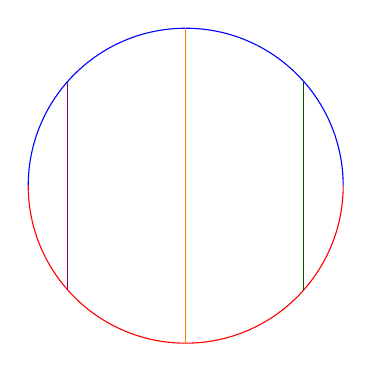
\begin{tikzpicture}
    \draw[red] (-2,0) arc (180:360:2);
    \draw[blue] (2,0) arc (0:180:2);
    \draw[green!30!black] (1.5,1.32) -- (1.5,-1.32);
    \draw[orange] (0,2) -- (0,-2);
    \draw[violet] (-1.5,1.32) -- (-1.5, -1.32);
\end{tikzpicture}
\qquad \qquad \qquad  
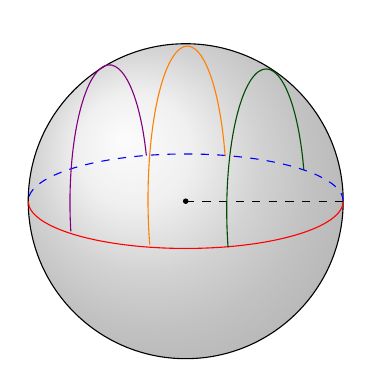
\begin{tikzpicture}
    \shade[ball color = gray!40, opacity = 0.4] (0,0) circle (2cm);
  \draw (0,0) circle (2cm);
  \draw[red] (-2,0) arc (180:360:2 and 0.6);
  \draw[dashed,blue] (2,0) arc (0:180:2 and 0.6);
  \draw[dashed] (0,0 ) -- (2,0);
  \fill[fill=black] (0,0) circle (1pt);
  \draw[green!30!black] (1.5,0.39686) arc (16.699:195:0.5 and 1.8);
  \draw[orange] (0.5,0.58) arc (16.699:197:0.5 and 1.95);
  \draw[violet] (-0.5,0.58) arc (20:192: 0.5 and 1.75);
\end{tikzpicture}
    \end{equation*}
    Wir erhalten das Diagramm:
    \begin{equation*}
    \begin{tikzcd}
        D^n \ar{r} \ar{d} & S^n \ar{d} \\
    D^n / \sim \ar[dashed,swap]{r}{\overline{f}} & S^n / (x\sim -x) \cong \R\mathbb{P}^n
    \end{tikzcd}
    \end{equation*}
    Wir sehen leicht, dass $\overline{f}$ bijektiv ist. Da $D^n$ kompakt, ist auch  $D^n / \sim $ kompakt, und $\R\mathbb{P}^n$ ist Hausdorffsch, also handelt es sich um einen Homöomorphismus (mit \autoref{cor:stetige-bijektion-von-kompaktem-raum-in-hausdorff-raum-ist-homöomorphismus})
\end{proof}

\begin{corollary}\label{cor:quotientenraum-von-kompaktem-hausdorffraum-mit-teilmenge-ist-hausdorff-gdw-teilmenge-abgeschlossen}
    Sei $X$ kompakt und Hausdorffsch und  $A\subset X$. Dann sind äquivalent
    \begin{enumerate}[1)]
        \item $X / A$ ist Hausdorffsch
        \item  $A$ ist abgeschlossen.
    \end{enumerate}
\end{corollary}
\begin{proof}
    '$1)\implies_2)$'. Ist $X / A$ Hausdorffsch, so ist die einpunktige Menge $\left \{[A]\right\}$ abgeschlossen (nach \autoref{thm:hausdorff-impliziert-t1}). Also ist $q^{-1}(A) = A$ abgeschlossen nach Definition der Quotiententopologie. \\
    '$2)\implies 1)$' Nach \autoref{thm:quotientenraum-von-hausdorffraum-ist-hausdorff-gdw-projektion-abgeschlossen} genügt es zu zeigen, dass $q: X \to  X / A$ abgeschlossen ist. Für $B\subset X$ abgeschlossen ist, müssen wir also zeigen, dass $q(B)$ abgeschlossen ist, nach Definiton also, dass  $q^{-1}(q(B))\subset X$ abgeschlossen ist. Nun ist
    \[
        q^{-1}(q(B)) = \begin{cases}
            B & \text{falls } B\cap A = \emptyset \\
            B \cup A & \text{falls }B \cap  A \neq  \emptyset
        \end{cases}
    .\] 
    abgeschlossen, weil $A$ abgeschlossen ist. 
\end{proof}


\begin{example}
    \begin{enumerate}[a)]
        \item
Es ist $D^n / S^{n-1}$   Hausdorffsch. Alternativ können wir auch sehen, dass $D^n / S^{n-1} \cong S^n$ ist. Hierzu betrachte die Projektion:
    \begin{equation*}
    \begin{array}{c c l} 
    D^n & \longrightarrow & S^n \\
    x & \longmapsto &  \begin{cases}
        (2x, \sqrt{1-\lVert 2x \rVert ^2} & 0 \leq  \lVert x \rVert \leq \frac{1}{2}  \\
        \left( \frac{2-2\lVert x \rVert }{\lVert x \rVert }\cdot x, - \sqrt{1-(2-2\lVert x \rVert )^2}  \right) & \frac{1}{2} \leq  \lVert x \rVert  \leq 1
    \end{cases}
    \end{array}
\end{equation*}
Diese ist stetig, denn falls $\lVert x \rVert =\frac{1}{2}$ ist
\[
\frac{2-2\lVert x \rVert }{\lVert x \rVert } = \frac{2-1}{\frac{1}{2}} = 2
.\] 
und
\[
    \sqrt{1-\lVert 2x \rVert ^2} = \sqrt{1-1} =0 = - \sqrt{0} = -\sqrt{1-(2-2\lVert x \rVert )^2}  
.\] 
Ist $\lVert x \rVert =1$, so ist
 \[
\frac{2-2\lVert x \rVert }{\lVert x \rVert } = 0
.\] 
und somit ist $f(x) = (0,-1) \in \R^n \times \R$. Also faktorisiert $f$ über  $\overline{f} : D^n / S^{n-1} \to  S^n$. Wir sehen wieder leicht, dass $\overline{f}$ stetige Bijektion ist. Da $D^n / S^{n-1}$ kompakt und $S^n$ Hausdorffsch, folgt wieder, dass  $\overline{f}$ ein Homöomorphismus ist. \\
\item Wir erhalten nun eine Abbildung:
    \[
    \begin{tikzcd}
        S^n \ar{r}{q} & S^n / (x\sim -x) \cong \R\mathbb{P}^n \cong D^n / (x\sim -x) \ar{r} &  D^n / S^{n-1} \cong S^n
    \end{tikzcd}
\]
und diese ist im Allgemeinen \underline{kein} Homöomorphismus, denn jeder Punkt hat 2 Urbilder.
    \end{enumerate}
\end{example}
\todo{Abbildung skizzieren}

\def\Base{\mathcal{S}} %temporary
\section{Basen und Subbasen}
\begin{definition}[Basis]\label{def:basis}
    Sei $(X, \mathcal{O})$ ein topologischer Raum. Sei $\Base \subset \mathcal{O}$ eine Menge offener Mengen. Dann heißt $\Base$
    \begin{description}
        \item[\vocab{Basis}], falls $\forall U\subset \mathcal{O}$ existiert $S_i \in \Base$ mit $U = \bigcup_{i\in I} S_i$ 
        \item[\vocab{Subbasis}], falls $\forall U\in \mathcal{O}$ existieren $I, K_i$ endlich sowie  $S_k \in  \Base$ mit 
            \[
            U = \bigcup_{i\in I} \bigcap_{k\in K_i} S_k 
            .\] 
    \end{description}
\end{definition}
\begin{remark}
Ist     $\Base$ eine Basis, so ist $\Base$ eine Subbasis.
\end{remark}
\begin{example}
    Ist $(X,d)$ ein metrischer Raum, so ist
     \[
         \Base = \left \{U(x,ε) \mid  x\in X, ε>0\right\} 
    .\] 
    eine Basis der Topologie.
\end{example}
\begin{theorem}[Erzeugte Topologie]\label{thm:erzeugte-topologie}
    Sei $X$ eine Menge,  $\Base \subset \mathcal{P}(X)$ eine Menge von Teilmengen. Dann existiert genau eine Topologie auf  $X$, für die  $\Base$ eine Subbasis ist, nämlich:
     \[
    \mathcal{O} = \left \{U\subset X \mid  U = \bigcup_{i \in  I} \bigcap_{k\in K_i} S_k \text{ mit } \abs{K_i}<\infty, S_k \in  \Base  \right\} 
    .\] 
\end{theorem}
\begin{proof}
    Übung als \autoref{aufgabe-3.2}.
\end{proof}
\begin{dnotation}
    Wir nennen $\mathcal{O}$ die \vocab[Topologie!von $\Base$ erzeugte]{von $\Base$ erzeugte Topologie}.
\end{dnotation}

\begin{lemma}[Stetigkeit auf Subbasiselementen]\label{lm:stetigkeit-auf-subbasis}
    Sei $f: X \to  Y$ eine Abbildung zwischen topologischen Räumen, $\Base$ eine Subbasis von $Y$. Dann sind äquivalent:
    \begin{enumerate}[1)]
        \item $f$ ist stetig
        \item  $f^{-1}(S)$ ist offen für alle $S\in \Base$
    \end{enumerate}
\end{lemma}

\begin{proof}
    '$1) \implies 2)$' ist klar, da Subbasiselemente offen sind. \\
    '$2) \implies 1)$'. Sei $U \subset Y$ offen, dann $\exists K_i$ endlich und $S_k \in \Base$ mit
    \[
    U = \bigcup_{i \in  I} \bigcap_{k\in K_i} S_k
    .\] 
    Dann ist aber genau
    \[
        f^{-1}(U) = \bigcup_{i \in  I} \bigcap_{k\in K_i} \underbrace{f^{-1}(S_k)}_{\text{offen}} 
    .\] 
    offen, weil endliche Schnitte und beliebige Vereinigung offener Mengen offen sind. Also ist $f$ stetig.
\end{proof}

\begin{theorem}\label{thm:subbasis-ist-basis-wenn-schnitt-generiert-wird}
    Eine Subbasis $\Base$ von  $(X, \mathcal{O})$ ist eine Basis genau dann, wenn
    \[
    \forall S_1, S_2 \in \Base \;\exists S_i \in \Base \colon S_1 \cap S_2 = \bigcup_{i \in I} S_i
    .\] 
\end{theorem}


\begin{proof}
'$\implies$'    Da $S_1,S_2 \in \Base$ sind diese offen. Dann ist auch $S_1\cap S_2$ offen. Ist $\Base$ Basis, dann gibt es also  $S_i \in  \Base$ mit 
\[
S_1 \cap  S_2 = \bigcup_{i \in  I} S_i
.\] 
'$\impliedby$' Angenommen, $U\subset X$ ist offen und von der Form
\[
    U = \bigcup_{i \in  I} \left( \bigcap_{k\in K_i} S_k \right) 
.\] 
mit $K_i$ endlich und  $S_k \in  \Base$. Nach Annahme ist
\[
\bigcap_{k\in K_i} = \bigcup_{j\in J_i} S_j  
.\] 
und damit ist
\[
U = \bigcup_{i\in I} \bigcup_{j\in J_i} S_j  
.\] 
\end{proof}
\begin{remark*}
    Nach Annahme ist eigentlich erstmal der Schnitt von 2 Mengen die Vereinigung von $S_i$. Allerdings kann man dies per Induktion leicht auf  $n$ Teilmengen verallgemeinern, wenn wir
     \[
         \bigcap_{k=1}^n S_k = S_1 \cap  \bigcap_{k=2}^{n} S_k = S_1 \cap \bigcup_{i\in I} S_i = \bigcap_{i\in I} (S_i \cap S_k) = \bigcup_{i\in I} \bigcup_{j\in J_i} S_j  
    .\]
    für geeignete $S_i, S_j\in \Base$ schreiben.
\end{remark*}
\begin{theorem}[Satz von Alexander]\label{thm:alexander}
    Sei $X$ ein topologischer Raum und  $\Base$ eine Subbasis. Dann ist  $X$ kompakt genau dann, wenn jede Überdeckung durch Elemente aus  $\Base$ eine endliche Teilüberdeckung besitzt.
\end{theorem}
\begin{proof}
    '$\implies$' ist klar. \\
    '$\impliedby$' Angenommen, $X$ ist nicht kompakt, dann betrachte die Menge
     \[
    \mathcal{C} := \left \{U \mid  U \text{ offene Überdeckung \underline{ohne} endliche Teilüberdeckung}\right\} \neq \emptyset
    .\] 
    Es ist $\mathcal{C}$ partiell geordnet, indem wir $U\leq U'$ für $U\subset U'$ setzen. \\
    Ist $U_1\subset U_2\subset \ldots$ eine Kette, so ist $\bigcup_{U_i}\in \mathcal{C}$, denn
    \begin{itemize}
        \item Offenbar ist $\bigcup_{i \in  I} U_i$ eine offene Überdeckung.
        \item Hat $\bigcup_{i \in  I} U_i$ eine endliche Teilüberdeckung, so ist diese schon in einem $U_i$ enthalten, und damit enthielte auch dieses  $U_i$ bereits eine endliche Teilüberedckung \contra
    \end{itemize}
Wir können also das Lemma von Zorn anwenden, und somit existiert ein maximales Elment $U\in \mathcal{C}$.
\begin{claim}
    Ist $V\subset X$ offen und  $V\not\in U$, so hat $U\cup \left \{V\right\} $ eine endliche Teilüberdeckung
\end{claim}
\begin{subproof}
    Sonst wäre $U \cup \left \{V\right\} \in \mathcal{C}$ und somit wäre $U$ nicht maximal
\end{subproof}
\begin{claim}
    $U \cap \Base$ ist keine Überdeckung
\end{claim}
\begin{subproof}
    Sonst hätte $U$ eine endliche Teilüberedckung nach Annahme.
\end{subproof}
Wegen Behauptung 2 existiert $x\in X$, der nicht von $U \cap \Base$ überdeckt wird. Sei $W\in U$ mit $x\in W$. Da $W$ offen ist, folgt
 \[
W = \bigcup_{i \in  I} \bigcap_{k\in K_i} S_k
.\] 
mit $K_i$ endlich und  $S_k \in \Base$. Dann existieren also $S_1,\ldots,S_n$ mit 
\[
x \in  \bigcap_{i=1}^n S_i \subset W 
.\] 
Da $x$ nicht von  $U \cap \Base$ überdeckt wird, ist $S_i \not\in U$. Aus der ersten Behauptung wissen wir nun aber, dass es $U_1^i, \ldots, u_{n_i}^i \in U$ mit
\[
\left \{U_j ^i\right\} _{j=1}^n \cup \left \{S_i\right\}  \quad \text{ ist Überdeckung von } X
.\] 
Sei nun 
\[
\hat{U} := \left \{U_j ^i \mid  1\leq i\leq n, 1\leq j\leq n_i\right\} \subset U
.\] 
Für alle $i$ gilt also
 \[
X \subset \bigcup_{V\in \hat{U}} V \cup S_i 
.\] 
Also folgt
\[
X \setminus \bigcup_{V\in \hat{U}} V \subset S_i 
.\] 
und damit ist auch
\[
X\setminus \bigcup_{V\in \hat{U}} V \subset S_1 \cap \ldots \cap S_n \subset W \in U 
.\] 
Also ist $\hat{U}\cup \left \{W\right\} $ eine endliche Teilüberdeckung von $U$, \contra.
\end{proof}

    \lecture{6}{Sa 01 Mai 2021 09:18}{Erwartungswert von Zufallsvariablen,Varianz}
\begin{example}[Zufallsvariablen mit Werten in $\left\{0,1\right\}$]
    Sei $A\in \mathcal{F}$ ein Ereignis, und definiere $X$ durch
     \[
         X(\omega) := \mathbbm{1}_{A}(\omega) = \begin{cases}
             1 & \text{falls } \omega\in A \\
             0 & \text{sonst}
         \end{cases}
    .\] 
    Dann ist
    \[
        \mathbb{E}(X) = \mathbb{P}(A)
    .\] 
    \begin{proof}
        Nach Definition ist
        \begin{equation*}
            \begin{split}
                \mathbb{E}(X) &= 0\cdot  \mathbb{P}(X= 0) + 1\cdot \mathbb{P}(X=1)  \\
                              &= \mathbb{P}(A)
            \end{split}
        \end{equation*}
    \end{proof}
\end{example}
\begin{example}[Binomialverteilung]
    Sei $X\sim \Bin(n,p)$. Wir wollen zeigen, dass $\mathbb{E}(X) = p\cdot n$.
    \begin{proof}
        \[
            \mathbb{E}(X) = \sum_{k=0}^n \underbrace{\binom{n}{k} p^k (1-p)^{n-k}}_{=\mathbb{P}(X=k)} \cdot k
        .\]
        Wir wollen nun allgemein, in Anlehnung an die Binomialformel, den Wert von
        \[
            \sum_{k=0}^n \binom{n}{k} p^k q^{n-k}\cdot k
        .\] 
berechnen. Dazu stellen wir fest, dass
\[
    p\cdot \frac{d}{dp} \sum_{k=0}^n \binom{n}{k}p^{k} q^{n-k} = p\cdot \sum_{k=0}^n \binom{n}{k} p^{k-1}q^{n-k}\cdot k
.\] 
unser Ausdruck ist, also suchen wir
\[
    p\cdot \frac{d}{dp}(p+q)^n = p\cdot (p+q)^{n-1}\cdot n
.\] 
Nun können wir $q=1-p$ auf beiden Seiten setzen, und somit erhalten wir
 \[
     \mathbb{E}(X) = p\cdot (p+(1-p))^{n-1}\cdot n = p\cdot n
.\] 
wie gewünscht.
    \end{proof}
\end{example}
\begin{example}[Poisson-Verteilung]
    Sei $X\sim \Poi(λ)$, dann behaupten wir, dass $\mathbb{E}(X) = λ$.
    \begin{proof}
        \[
            \begin{split}
                \mathbb{E}(X) &= \sum_{k\geq 0} \frac{e^{-λ} λ^k}{k!} \cdot k \\
            &=e^{-λ} \cdot λ\cdot \underbrace{\sum_{k\geq 1} \frac{λ^{k-1}}{(k-1)!}}_{\to e^{λ}} \\
            &= λ
            \end{split}
        .\] 
    \end{proof}
\end{example}
\begin{remark*}
    Diese Feststellung passt auch zur Konstruktion der Poisson-Verteilung.
\end{remark*}
\begin{remark}
    Oft kann man definieren
    \[
        \psi (z) := \sum_{k\in \mathcal{S}} p(k) z^k
    .\] 
    Dann werden wir uns 
    \[
        \frac{d}{dz}\psi (z) = \sum_{k\in \mathcal{S}} p(k)kz^{k-1}
    \]
    ansehen und bei $z=1$ evaluieren, um  $\mathbb{E}(X)$ zu berechnen. \\
    Das ganze funktioniert, wenn $X$ durch  $\mathbb{P}(X=k) = p(k)$ verteilt ist und natürlich nur, wenn alle Objekte wohldefiniert sind.
\end{remark}
Wir wollen auch Funktionen von $X$ betrachten.
\begin{figure}[ht]
    \centering
    \incfig{funktionen-von-zufallsvariablen}
    \caption{Funktionen von Zufallsvariablen}
    \label{fig:funktionen-von-zufallsvariablen}
\end{figure}
\begin{theorem}[Transformationssatz]\label{thm:transformationssatz}
    Sei $X:\Omega\to \mathcal{S}$ eine diskrete Zufallsvariable und $f: \mathcal{S} \to  \R$ eine Funktion. Dann ist $f(X) := f \circ  X \colon \Omega\to \R$ auch eine Zufallsvariable und 
    \[
        \mathbb{E}(f(X)) = \sum_{s\in \mathcal{S}} f(s) \mathbb{P}(X=s)
    .\] 
    falls die Summe wohldefiniert ist.
\end{theorem}
\begin{proof}
    Messbarkeit: Es ist
    \[
        \left \{f(X) = a\right\}  = \bigcup_{s\in f^{-1}(a)} \left \{X=s\right\}  \in \mathcal{F}
    .\] 
    weil
    \[
        \left \{\omega \mid  X(\omega) = s\right\} \in \mathcal{F}
    .\] 
    da $X$ eine Zufallsvariable ist. Nach Definition ist nun
    \begin{equation*}
        \begin{split}
            \mathbb{E}(f(X)) &= \sum_{a\in f(\mathcal{S})} a\cdot \mathbb{P}(f(X)=a) \\
                             &= \sum_{a\in f(\mathcal{S})} a\cdot \mathbb{P}\left( \bigcup_{s\in f^{-1}(a)} \left \{X=s\right\}   \right) \\
                             &=\sum_{a\in f(\mathcal{S})} a\cdot \sum_{s\in f^{-1}(a)} \mathbb{P}(X=s) \\
                             &=\sum_{a\in f(\mathcal{S})} \sum_{s\in f^{-1}(a)} f(s) \mathbb{P}(X=s) \\
                             &= \sum_{s\in \mathcal{S}} f(s) \mathbb{P}(X=s)
        \end{split}
    \end{equation*}
\end{proof}

Der Erwartungswert ist {\sc Linear} und {\sc Monoton}:
\begin{theorem}[Linearität des Erwartungswerts]\label{thm:linearität-des-erwartungswerts}
    Seien $X_1:\Omega\to \mathcal{S}_1$ und $X_2:\Omega\to \mathcal{S}_2$ zwei diskrete Zufallsvariablen auf $(\Omega,\mathcal{F},\mathbb{P})$. Falls $\mathbb{E}(\abs{X_1})<\infty $ und $\mathbb{E}(\abs{X_2})<\infty $, dann ist $\forall λ_1,λ_2\in \R$:
    \[
        \mathbb{E}(λ_1 X_1 + λ_2 X_2) = λ_1 \mathbb{E}(X_1) + λ_2 \mathbb{E}(X_2)
    .\] 
\end{theorem}
\begin{proof}
    Es ist
    \[
        \abs{\mathbb{E}(λ_1 X_1 + λ_2 X_2)} \leq  \abs{λ_1} \mathbb{E}(\abs{X_1}) + \abs{λ_2} \mathbb{E}(\abs{X_2}) < \infty     
    .\] 
    (nach Dreiecksungleichung). Nun rechnen wir aus:
    \[
        \mathbb{E}(λ_1 X_1 + λ_2 X_2) = \mathbb{E}(f(X_1,X_2))
    .\] 
    wobei $f(x_1,x_2) = λ_1 x_1 + λ_2x_2$, also
    \[
        \begin{split}
        &= \sum_{\substack{ x_1\in \mathcal{S}_1\\x_2\in \mathcal{S}_2}}f(x_1,x_2) \mathbb{P}(X_1=x_1 \cap X_2 = x_2) \\
        &= λ_1 \sum_{x\in \mathcal{S}_1} x_i \sum_{x_2\in \mathcal{S}_2} \mathbb{P}(X_1=x_1 \cap X_2 = x_2) + \text{sym.} \\
        &= λ_1 \sum_{x\in \mathcal{S}_1} x_i \mathbb{P}(X_1 = x_1) + \text{sym.} \\
        &=λ_1\mathbb{E}(X_1) + λ_2 \mathbb{E}(X_2)
        \end{split}
    .\] 
\end{proof}
\begin{corollary}[Monotonie des Erwartungswerts]\label{cor:erwartungswert-ist-monoton}
    Seien $X_1,X_2$ reellwertige Zufallsvariablen mit $X_1(\omega) \leq  X_2(\omega)$ für alle $w\in \Omega$. Dann ist
    \[
        \mathbb{E}(X_1) \leq  \mathbb{E}(X_2)
    .\] 
\end{corollary}
\begin{proof}
    Da $X_2(\omega) - X_1(\omega) \geq 0$, also ist trivialerweise $\mathbb{E}(X_2-X_1)\geq 0$. Wegen der Linearität ist nun $\mathbb{E}(X_2-X_1) = \mathbb{E}(X_2) - \mathbb{E}(X_1)$ und somit sind wir fertig.
\end{proof}
\begin{example}
    Seien $A_1,A_2,\ldots,A_n \in \mathcal{F}$ mit $\mathbb{P}(A_i) = p$ für alle $i$. Sei  $X_i := \mathbbm{1}$. Dann ist $X_i \sim \Ber(p)$ und $\mathbb{E}(X_i) = p$. Sei
    \[
    \mathcal{S}_n := \sum_{i=1}^n X_i
    .\] 
    Dann ist
    \[
        \mathbb{E}(\mathcal{S}_n) = \sum_{i=1}^n \mathbb{E}(X_i) = \sum_{i=1}^n p = np
    .\] 
    Das ist eine Verallgemeinerung des Falles, in dem  $A_1,\ldots,A_n$ unabhängig sind, weil dann $\mathcal{S}_n \sim  \Bin(n,p)$.
\end{example}
Oft interessieren wir uns auch dafür, wie weit eine Zufallsvariable von ihrem Ursprungswert entfernt ist. Ist z.B. $\mathbb{P}(X=k) = \mathbb{P}(X=-k)$, so ist $\mathbb{E}(X) = 0$, so sind immer noch folgende Fälle denkbar:
\todo{Plot einfügen}
\begin{question}
    Wie weit sind die Werte vom $X$ Mittelwert ($\mathbb{E}(X)$) entfernt?
\end{question}
Die Antwort liefert die sogenannte Varianz $\Var(X)$:
\begin{definition}[Varianz]\label{def:varianz}
    Sei $X$ eine reellwertige Zufallsvariable auf  $(\Omega,\mathcal{F},\mathbb{P}\mathbb{P})$ mit $\mathbb{E}(X^2)<\infty$. Die \vocab{Varianz} von $X$ ist durch
    \[
        \Var(X) := \mathbb{E}((X-\mathbb{E}(X))^2)
    .\] 
    definiert.
\end{definition}
Eigenschaften der Varianz:
\begin{enumerate}[label=\protect\circled{\alph*}]
    \item Klarerweies ist $\Var(X) \geq 0$. Dazu $\Var(X) = 0 \iff  \mathbb{P}(X = \mathbb{E}(X)) = 1$, d.h. $X(\omega)$ ist eine Konstante.
        \item Linearität impliziert, dass
            \[
                \Var(X) = \mathbb{E}(X^2) - \left( \mathbb{E}(X) \right) ^2 \qquad \Var(λ\cdot X) = λ^2\Var(X)
            .\] 
        \item Die Varianz hängt nicht von dem Erwartungswert ab, d.h.
            \[
                \Var(X) = \Var(X+a) \qquad \forall a\in \R
            .\] 
\end{enumerate}
\begin{example}
    \begin{enumerate}[label=\protect\circled{\alph*}]
        \item Ist $X\sim \Ber(p)$, so ist $\Var(X) = p(1-p)$.
        \item Ist  $X\sim \Bin(n,p)$, so ist $\Var(X) = n\cdot p(1-p)$.
        \item Ist $X\sim \Poi(λ)$, so ist $\Var(X) = λ$
        \item Ist  $X\sim \Geo(q)$, so ist $\Var(X) = \frac{q}{(1-q)^2}$
    \end{enumerate}
\end{example}
\begin{proof}
    \begin{enumerate}[label=\protect\circled{\alph*}]
        \item Wir benutzen $\Var(X) = \mathbb{E}(X^2) - (\mathbb{E}(X))^2$. Nun ist
            \[
                \mathbb{E}(X^2) = 0^2 \mathbb{P}(X=0) + 1^2\mathbb{P}(X=1) = p
            .\] 
            und somit $\Var(X) = p-p^2 = p(1-p)$
        \item Sei $X\sim \Bin(n,p)$, wir wissen bereits $\mathbb{E}(X) = p\cdot n$. Nun ist
            \[
                \mathbb{E}(X^2) = \sum_{k=0}^n \binom{n}{k} p^k (1-p)^{n-k} k^2
            .\]
            Wir benutznen den gleichen Trick wie vorher nochmal, indem wir feststellen:
            \[
                \begin{split}
                    \sum_{k=0}^n \binom{n}{k} p^k q^{n-k}k^2 &= \sum_{k=0}^n \binom{n}{k} p^{k} q^{n-k} k (k-1) + \sum_{k=0}^n \binom{n}{k} p^{k} q^{n-k}k \\
                                                             &= p^2 \frac{d^2}{dp^2} (p+q)^n + p \frac{d}{dp} (p+q)^n \\
                                                             &= p^2(p+q)^{n-1}n(n-1) + p(p+q)^{n-1}\cdot n
                \end{split}
            .\] 
            Einsetzen von $q=1-p$ liefert nun:
             \[
                 \mathbb{E}(X^2) = p^2n(n-1) + p\cdot n = p^2n^2 - p^2n + pn
            .\] 
            Damit erhalten wir schlussendlich
            \[
                \Var(X) = p^2n^2 - p^2n + pn - (pn)^2 = np(1-p)
            .\] 
        \item Ist $X\sim \Poi(λ)$, so wissen wir beretis $\mathbb{E}(X) = λ$. Nun ist
            \[
                \begin{split}
                    \mathbb{E}(X^2) &= \sum_{k\geq 0} k^2 \cdot  \frac{e^{-λ}λ^k}{k!} = \sum_{k\geq 0}k(k-1)\frac{e^{-λ}λ^k}{k!} + \sum_{k\geq 0} k \frac{e^{-λ}λ^k}{k!} \\
                &=λ^2e^{-λ}\sum_{k\geq 2} \frac{λ^{k-2}}{(k-2)!} + e^{-λ}λ\sum_{k\geq 1}\frac{λ^{k-1}}{(k-1)!} \\
                &= λ^2+λ
                \end{split}
            .\] 
            Und damit ergibt sich für die Varianz:
            \[
                \Var(X) = λ^2 + λ - (λ) ^2 = λ
            .\] 
    \end{enumerate}
\end{proof}
\begin{remark}
    Sei $X:\Omega\to \mathcal{S}$ eine Zufallsvariable. Wir beobachten $X$  $n$ mal. Der Erwartungswert des Empirischen Masses ist genau der empirische Mittelwert, also für Beobachtungen $x_1,\ldots,x_n$ genau
    \[
    m_n := \frac{1}{n} \sum_{i=1}^n x_i
    .\] 
\end{remark}
\begin{example}[Anwendung]
    Ein alternativer Beweis des \nameref{cor:einschluss-ausschluss-prinzip}s lässt sich mit der Linearität des erwartungswerts führen:\\
Es ist
\[
    \begin{split}
    \mathbb{P}((A_1 \cup \ldots\cup A_n)^{c}) &= \mathbb{P}(A_1^{c}\cap \ldots\cap A_n^{c}) \\
                                              &= E(1_{A^{c}\cap \ldots\cap A_n^{c}}) = (1_{A_1^{c}}\cdot \ldots\cdot 1_{A_n^{c}}) \\
                                              &= E((1-1_A)\cdot \ldots\cdot (1-1_{A_n})) \\
                                              &\stackrel{\text{Linearität}}{=} \sum_{k=0}^n (-1)^k \sum_{1\leq i_1<\ldots<i_k\leq n} \mathbb{E}(1_{A_{i_1}}\cdot \ldots\cdot 1_{A_{i_k}}) \\
                                              &=\sum_{k=0}^n (-1)^k \sum_{1\leq i_1<\ldots<i_k\leq n}\mathbb{P}(A_{i_1}\cap \ldots\cap A_{i_k})
    \end{split}
.\] 
Komplementbildung liefert nun das gewünschte Ergebnis:
\[
    \begin{split}
    \mathbb{P}(A_1\cup \ldots\cup A_n) &= 1-\mathbb{P}((A_1\cap \ldots\cap A_n)^{c}) \\
                                       &= \sum_{k=1}^n (-1)^{k-1} \sum_{1\leq i_1<\ldots<i_k\leq n} \mathbb{P}(A_{i_1}\cap \ldots\cap A_{i_k})
    \end{split}
.\] 
\end{example}

    \lecture[Universelle Eigenschaft unendlicher Produkte. Satz von Tychonoff. Abschluss, Dichtheit. Einbettungen. Kompaktifizierung. Vollständige Regularität. Universelle Eigenschaft der Stone-Čech-Kompaktifizierung. Fortsetzung stetiger Funktionen.]{Di 04 Mai 2021 12:12}{Kompaktifizierung}

\begin{theorem}[Universelle Eigenschaft des Produkts]\label{thm:universelle-eigenschaft-des-produkts}
    Seien $(X_i)_{i\in I}$ topologische Räume, $A$ ein topologischer Raum und seien $f_i : A \to  X_i$ Funktionen. Sei
        \begin{equation*}
        f: \left| \begin{array}{c c l} 
        A & \longrightarrow & \prod_{i \in I} X_i \\
        a & \longmapsto &  (f_i(a))_{i \in I}
        \end{array} \right.
    \end{equation*}
    Dann ist $f$ stetig genau dann, wenn alle  $f_i$ stetig sind.
    \[
    \begin{tikzcd}
        & & X_1 \\
        & & X_2 \\
    A \ar[dashed]{r}{f} \ar[bend left = 40]{uurr}{f_1} \ar[bend left = 20]{urr}{f_2} \ar[bend right = 20,swap]{drr}{f_i} \ar[dashed, bend right = 40]{ddrr}& \prod_{i \in I}X_i \ar[near end]{uru}{\pr_1} \ar[swap]{ur}{\pr_2} \ar{dr}{\pr_i} \ar[bend right = 20,dashed]{ddr} \ar[dashed]{r}& \vdots \\
          & & X_i \\
          & & \vdots
    \end{tikzcd}
    .\] 
\end{theorem}
\begin{remark*}
    Die Universelle Eigenschaft ist genau genommen die Folgende: \\
    Seine $(X_i)_{i \in I}$ topologische Räume. Ein topologischer Raum $X$  zusammen mit Abbildung  $\pr_i : X \to  X_i$ wird Produkt der $X_i$ genannt, wenn es für jedes  $A$ und stetige Abbildungen  $f_i : A \to  X_i$ genau eine induzierte Abbildung $f: A \to  X$ gibt. \\
    Diese Eigenschaft ist nun universell im Sinne der Kategorientheorie, d.h. bis auf eindeutig bestimmten Isomorphismus gibt es nur ein Paar $(X, (\pr_i)_{i \in I})$, das die oben genannten Eigenschaften bestimmt. \\
    Wir haben zwar oben nicht die Eindeutigkeit des Produkts gezeigt, aber dessen Existenz (was aus der Kategorientheorie nicht ohne weiteres folgt), indem wir ein explizites solches Objekt konstruiert haben.
\end{remark*}
\begin{remark*}
    Insbesondere sollte man sich merken, dass die kanonischen Projektionen $\pr_i$ wichtiger Teil der Information eines Produktes sind. Bei unsere expliziten Konstruktion 'kanonisch', denkbar ist jedoch auch, eine völlig andere Trägermenge des Produkts zu wählen, dann ist die Angabe der Projektionen essentiell.
\end{remark*}
\begin{proof}
    '$\implies$' Sei $j\in I$, setze
        \begin{equation*}
        pr_j: \left| \begin{array}{c c l} 
        \prod_{i\in I}  & \longrightarrow & X_j \\
        (x_i)_{i \in I} & \longmapsto &  x_j
        \end{array} \right.
    \end{equation*}
    als Projektion auf die $j$-te Komponente.
     \begin{claim}
        $\pr_j$ ist stetig
    \end{claim}
    \begin{subproof}
        Ist $U\subset X_j$ offen, dann ist $pr_j^{-1}(U) = U\times \prod_{i\neq j} X_i\in \mathcal{S}$ ein Element der Subbasis der Produkttopologie, also offen. Also ist $pr_j$ stetig.
    \end{subproof}
    Nun ist $f_j = pr_j \circ  f$ stetig als Verknüpfung stetiger Funktionen.
    \begin{recap}
        \emphasize{Verknüpfungen stetiger Funktionen sind stetig:}\\
        Seien $f:X\to Y$ und $g:Y\to Z$ stetig, dann ist $g\circ  f : X \to  Z$ stetig.
        \begin{proof}
            Ist $U\subset Z$ offen, so ist
            \[
                (g \circ  f) ^{-1}(U) = f^{-1}(g^{-1}(U)) \subset X
            .\] 
            offen, indem wir zunächst $g$ stetig und dann  $f$ stetig verwenden.
        \end{proof}
    \end{recap}
    '$\impliedby$' Es genügt zu zeigen, dass $f^{-1}(Y)\subset A$ offen ist für alle $Y\in \mathcal{S}$. Sei also solch ein $Y\in \mathcal{S}$ beliebig, dann ist dieses von der Form
    \[
    Y = U\times \prod_{i\neq j} X_i
    .\] 
    Dann ist $f^{-1}(Y) = f^{-1}_j(A)\subset A$ offen, da $f_j$ stetig ist.
\end{proof}
\begin{theorem}[Satz von Tychonoff]\label{thm:tychonoff}
    Sei $(X_i)_{i \in I}$ eine Familie kompakter Räume. Dann ist $\prod _{i \in I} X_i$ kompakt.
\end{theorem}
\begin{proof}
    Wir verwenden wieder den \nameref{thm:alexander} (\autoref{thm:alexander}). Sei $\mathcal{U}$ eine Überdeckung durch Elemente aus  $\mathcal{S}$. Sei $\mathcal{U}_j \subset \mathcal{U}$ gegeben durch die Elemente $V$ von  $\mathcal{U}$ der Form
    \[
    V = W \times \prod_{i\neq j} X_i \qquad \text{mit } W\subset X_j \text{ offen}
    .\] 
    Dann ist
    \[
    \mathcal{U} = \bigsqcup_{i \in  I} \mathcal{U}_j
    .\] 
    Ist nun
    \[
        \pr_i (\mathcal{U}_i)  = \left \{\pr_i(V) \mid  V\in \mathcal{U}_i\right\} 
    .\] 
    eine offene Überdeckung von $X_i$, so existiert - weil  $X_i$ kompakt - eine endliche Teilüberdeckung  $\pr_i(V_1)\cup \ldots\cup \pr_i(V_k)$ von $X_i$ mit  $V_j \in \mathcal{U}_i$. Dann ist $V_1,\ldots,V_k$ eine endliche Teilüberedckung von $\prod_{i \in I} X_i$. \\
    Wir sind also fertig, außer im Fall \\
    $\mathbb{A}$: $\pr_i(\mathcal{U}_i)$ ist  \underline{keine} Überdeckung von $X_i$ für alle  $i\in I$.  \\
    Dann finden wir $x_i \in X_i \setminus \bigcup_{V\in \mathcal{U}_i} \pr_i(V)$ für jedes $i\in I$. Dann ist aber der Punkt
    \[
        (x_i)_{i \in I}\in \prod_{i \in I}X_i
    .\] 
    nicht von $\mathcal{U}$ überdeckt: Ist $(x_i)_{i \in I} \in V\in \mathcal{U}$, dann gibt es $i\in I$ mit $V\in \mathcal{U}_i$, und daraus folgt bereits $x_i \in \pr_i(V)$, \contra.
\end{proof}
\begin{remark}
    Eigentlich haben wir die Notation $\pr_j$ für die Projektion  $\prod _{i \in I}X_i \to  X_j$ eingeführt, manchmal schreiben wir aber auch einfach nur $p_j$.
\end{remark}
\begin{example}
    \begin{enumerate}[a)]
        \item Seien $X_1,\ldots,X_n$ diskrete Räume. Dann ist auch $\prod_{i \in I}X_i$ diskret.
            \begin{proof}
                Es ist
                \[
                    \left \{(x_1,\ldots,x_n)\right\}  = \left \{x_1\right\} \times \ldots\times \left \{x_n\right\} 
                .\] 
                Element der Produkttopologie, weil die $\left \{x_i\right\} \subset X_i$ offen sind. Also sind alle Punkte offen.
            \end{proof}
        \item Betrachte $\left \{0,2\right\} $ mit der diskreten Topologie. Dann ist
            \[
            \prod_{\N} \left \{0,2\right\} =: \left \{0,2\right\} ^{\N}
            .\] 
            kompakt nach dem \nameref{thm:tychonoff}. Dann ist $\prod_{\N} \left \{0,2\right\} $ aber nicht diskret, weil wir sonst die offene Überdeckung
            \[
            \prod_{\N} \left \{0,2\right\} = \bigcup_{x\in \left \{0,2\right\} ^{\N}}  \left \{x\right\} 
            .\] 
            hätten, die keine endliche Teilüberdeckung besitzt.
    \end{enumerate}
\end{example}
\begin{remark*}
    Das Beispiel zeigt die wichtige Eigenschaft, dass \underline{nicht} (notwendigerweise) alle Mengen der Form $\prod_{i \in I}U_i$ für $U_i\subset X_i$ offen auch im Produkt $\prod_{i \in I}X_i$ offen sind.
\end{remark*}

\begin{theorem}\label{thm:produkte-von-Hausdorff-Räumen-sind-Hausdorff}
    Ist $\left \{X_i\right\} _{i \in I}$ eine Familie von Hausdorffräumen, so ist auch  $\prod _{i \in I} X_i$ Hausdorffsch.
\end{theorem}
\begin{proof}
    Ist $(x_i)_{i \in I} \neq  (y_i)_{i \in I} \in  \prod _{i \in I}X_i$, dann gibt es $i\in I$ mit $x_i \neq  y_i$. Da $X_i$ Hausdorffsch ist, existieren  $U_i, V_i \subset X_i$ offen mit $x_i \in U_i, y_i \in V_i$ und $U_i \cap  V_i = \emptyset$. Dann sind aber beretis
    \[
    U_i \times  \prod_{i\neq j} X_j \qquad V_i \times \prod_{i\neq j} X_j
    .\] 
    zwei disjunkte, offene Umgebungen von $(x_i)_{i \in I}$ und $(y_i)_{i \in I}$.
\end{proof}

\begin{goal*}
    Wir wollen uns im Folgenden Fragen, wann wir Räume in 'schöne' Räume einbetten können, wobei 'schön' für uns Kompakt + Hausdorff heißen soll.
\end{goal*}

\begin{definition}[Abschluss, Dichtheit] \label{def:abschluss-dichtheit}
    Sei $X$ ein topologischer Raum und $Y\subset X$ eine Teilmenge.
    \begin{enumerate}[1)]
        \item Der \vocab[Menge!Abschluss]{Abschluss} $\overline{Y}$ ist definiert als
            \[
            \overline{Y} := \bigcap_{\substack{Y\subset A \\ A\subset X \text{ abg.}} } A
            .\] 
            Als Schnitt abgeschlossener Mengen ist $\overline{Y}$ selbst abgeschlossen (wie der Name suggeriert).
        \item  $Y$ ist \vocab[Menge!dicht]{dicht} in $X$, falls  $\overline{Y} = X$.
    \end{enumerate}
\end{definition}
\begin{definition}[Einbettung]\label{def:einbettung}
    Sei $f:X\to Y$ stetig. Dann ist $f$ eine  \vocab{Einbettung}, falls $f: X \to  f(X)$ ein Homöomorphismus ist.
\end{definition}
\begin{definition}[Kompaktifizierung] \label{def:kompaktifizierung}
    Sei $ι: Y\hookrightarrow X$ eine Einbettung. Dann ist $X$ eine \vocab{Kompaktifizierung} von $Y$, falls
    \begin{enumerate}[1)]
        \item $X$ ist kompakt und Hausdorffsch.
        \item  $ι(Y)\subset X$ ist dicht (in $X$).
    \end{enumerate}
\end{definition}
\begin{definition}[Vollständige Regularität]\label{def:vollständig-regulär}
    Ein topologischer Raum $X$ ist  \vocab[Topologischer Raum!vollständig regulär]{vollständig regulär}, falls
    \begin{enumerate}[1)]
        \item $X$ ist Hausdorffsch
        \item  $\forall A\subset X$ abgeschlossen und $x\in X\setminus A$ existiert eine stetige Abbildung $f:X \to  [0,1]$, sodass $f(x) = 1$ und  $f\mid _A \equiv 0$
    \end{enumerate}
\end{definition}
\begin{remark}
    Jeder vollständig reguläre Raum ist regulär. Hierzu betrachte $f^{-1}\left( \left( \frac{1}{2},1 \right]  \right) $ sowie $f^{-1}\left( \left[ 0,\frac{1}{2}  \right)  \right) $. Diese sind offenbar disjunkt, offen, und Umgebungen von $x$ bzw.  $A$.
\end{remark}
\begin{lemma}\label{lm:teilraum-von-vollständig-regulärem-raum-ist-vollständig-regulär}
    Ist $X$ vollständig regulär und  $Y\subset X$, dann ist auch $Y$ vollständig regulär.
\end{lemma}
\begin{proof}
    \begin{enumerate}[1)]
        \item Da $X$ Hausdorffsch ist, ist auch  $Y$ Hausdorffsch.
        \item Sei  $A\subset Y$ abgeschlossen und $y\in Y \setminus A$. Dann existiert $A'\subset X$ abgeschlossen mit $A' \cap Y = A$. Da $X$ vollständig regulär ist,  gibt es  $f: X \to  [0,1]$ stetig mit $f\mid _{A'} \equiv  O$ und $f(y) = 1$. Dann erfüllt  $f\mid _Y : Y \to  [0,1]$ unsere gewünschten Bedingungen, weil
            \[
                \left(            f\mid _Y \right) \mid _A \equiv O \qquad f\mid _Y(y) = 1
            .\] 
    \end{enumerate}
\end{proof}
\begin{theorem}\label{thm:vollständig-regulär-wenn-kompaktifizierbar}
    $X$ ist genau dann vollständig regulär, wenn  $X$ eine Kompaktifizierung besitzt.
\end{theorem}
\begin{proof}
    Eine Richtung sei hier schon skizziert: ist $X$ kompakt und Hausdorffsch, so ist  $X$ normal (nach \autoref{thm:kompakter-hausdorff-raum-ist-normal}). Wir zeigen später, dass dann  $X$ auch vollständig regulär ist. Mit \autoref{lm:teilraum-von-vollständig-regulärem-raum-ist-vollständig-regulär} ist also $Y\subset X$ vollständig regulär.
\end{proof}
Konstruktion einer Kompaktifizierung: \\
Sei $X$ ein topologischer Raum. Sei 
\[
    \mathcal{C}(X) := \left \{f: X \to  [0,1] \mid  f \text{ stetig}\right\} 
.\] 
Nach \nameref{thm:tychonoff} ist $\prod_{\mathcal{C}(X)}[0,1] $ kompakt und nach \autoref{thm:produkte-von-Hausdorff-Räumen-sind-Hausdorff} Hausdorffsch. Definiere nun eine Abbildung
\[
    ι : X \to  \prod_{\mathcal{C}(X)} [0,1]
.\] 
durch die Komponenten $ι_f(x) = f(x)$. (wir benutzen also in der  $f$-ten Komponente einfach die Abbildung  $f$). Da alle  $f\in \mathcal{C}(X)$ stetig sind, ist $ι$ stetig (nach \autoref{thm:universelle-eigenschaft-des-produkts}). Setze nun
\[
    βX := \overline{ι(X)} \subset \prod_{\mathcal{C}(X)} [0,1]
.\] 
$β(X)$ ist kompakt und Hausdorffsch. $β(X)$ heißt  \vocab{Stone-Čech-Kompaktifizierung}. Diese ist jedoch nur eine Kompaktifizierung in \autoref{def:kompaktifizierung} falls $X$ vollständig regulär ist.
\begin{theorem}\label{thm:stone-cech-kompaktifizierung-ist-einbettung-für-vollständig-reguläre-räume}
     $ι: X \to  \prod_{\mathcal{C}(X)}[0,1]$ ist eine Einbettung, falls $X$ vollständig regulär ist.
\end{theorem}
\begin{proof}
    \textbf{Injektivität}: Seien $x\neq y\in X$. Dann sind $\left \{x\right\} ,\left \{y\right\} \subset X$ abgeschlossen und es existiert $f: X \to  [0,1]$ mit $f(x) = 0$ und  $f(y) = 1$. Dann ist aber bereits  $ι(x) \neq  ι(y)$ in Komponenten $f$. \\
    \textbf{Einbettung}: Wir müssen noch zeigen, dass $\forall  U\subset X$ offen $ι(U) \subset ι(X)$ offen ist, damit $ι : X \to  f(X)$ ein Homöomorphismus ist. \\
    Sei $U\subset X$ offen, setze $A := X\setminus U$ und sei $x\in U$. Dann finden wir (nach vollständiger Regularität von $X$) eine Funktion  $f: X \to  [0,1]$, sodass $f(x) = 1$ und  $f\mid _{A} = 0$. Setze
    \[
        V := \left( \frac{1}{2},1 \right]_f \times \prod_{\mathcal{C}(X) \setminus \left \{f\right\} } [0,1] \subset \prod_{\mathcal{C}(X)} [0,1]
    .\] 
    also offene Teilmenge von $\prod_{\mathcal{C}(X)} [0,1]$. Dann ist
    \[
        ι(x) \in \underbrace{V \cap  ι(X)}_{\text{offen in } ι(X)} \subset ι(X \setminus A) = ι(U)
    .\] 
    Damit ist $ι(U)\subset X$ Umgebung all seiner Punkte, also selbst offen.
\end{proof}
\begin{remark}
    Ist $K$ kompakt und Hausdorffsch, so ist  $ι(K) \subset \prod_{\mathcal{C}(K)} [0,1]$ kompakt, also abgeschlossen, da $\prod_{\mathcal{C}(K)} [0,1]$ kompakt, und deswegen ist $β(K) = ι(K) \cong K$.
\end{remark}
\begin{remark*}
    Der Homöomorphismus folgt daraus, dass wir (unter der noch nicht bewiesenen Annahme, dass normale Räume auch vollständig regulär sind) bereits wissen, dass es sich in diesem Fall bei $ι$ um eine Einbettung handelt.
\end{remark*}
\begin{lemma}[Fortsetzung stetiger Funktionen]\label{lm:fortsetzung-stetiger-funktionen-in-dichten-hausdorff-räumen-sind-eindeutig}
   Sei $f: X \to  Y$ stetig sowie $U\subset X$.
   \begin{enumerate}[1)]
       \item Dann ist $f(\overline{U}) \subset \overline{f(U)}$ 
       \item Ist $U\subset X$ dicht, $g: X\to Y$ auch stetig und $f\mid _ U = g\mid _U$ sowie $Y$ Hausdorffsch, so ist beretis  $f=g$
   \end{enumerate}
\end{lemma}
\begin{proof*}[Beweis]
    \begin{enumerate}[1)]
        \item Sei $y\in f(\overline{U})$, also gibt es $x\in \overline{U}$ mit $f(x) = y$. Sei  $y\in V\subset X$ eine beliebige offene Umgebung von $y$. Dann ist $f^{-1}(V)$ eine offene Umgebung von $x$ nach Stetigkeit von  $f$. Da  $x\in \overline{U}$ ist $f^{-1}(V)\cap U \neq \emptyset$ und wir wählen $x_0\in f^{-1}(V)\cap U$. Dann ist $f(x_0) \in V \cap f(U)$ und somit $V \cap f(U) \neq  \emptyset$. Da $V$ beliebig war, ist nach Definition  $y\in \overline{f(U)}$.
        \item Nimm an, dass $f\neq g$, dann gibt es $x\in X$ mit $f(x) != g(x)$. Da  $Y$ Hausdorffsch, können wir die beiden Punkte durch offene Mengen trennen, also finden wir  $f(x)\in U_f, g(x)\in U_g$ mit $U_f\cap U_g=\emptyset$ und $U_f,U_g$ offen. Dann sind auch $f^{-1}(U_f),g^{-1}(U_g)$ offene Mengen nach Stetigkeit von $f,g$, also ist auch  $f^{-1}(U_f)\cap g^{-1}(U_g)$ offen. Zudem $x\in f^{-1}(U_f)\cap g^{-1}(U_g)$, da $f(x)\in U_f,g(x)\in U_g$ nach Voraussetzung. Da $U\subset X$ dicht ist, ist $U\cap (f^{-1}(U_f)\cap g^{-1}(U_g))\neq \emptyset$ und wir finden $x_0\in U \cap  f^{-1}(U_f) \cap g^{-1}(U_g)$. Dann ist wegen $f\mid _{U}\equiv g\mid _{U}$ $f(x_0) = g(x_0)$, aber auch $f(x_0)\in U_f, g(x_0)\in U_g$, also $f(x_0) = g(x_0) \in U_f \in  U_g$. Aber nach Voraussetzung ist $U_f \cap  U_g = \emptyset$, \contra. Also $f\equiv g$.
\end{enumerate}
\end{proof*}
\begin{theorem}\label{thm:universelle-eigenschaft-der-stone-cech-kompaktifizierung}
    Sei $f: X \to  K$ stetig, $K$ kompakt und Hausdorffsch. Dann existiert eine eindeutige Fortsetzung $\hat{f}: β(X) \to  K$, so dass
    \[
   \begin{tikzcd}
       X \ar{r}{ι} \ar[swap]{d}{f} &  β(X) \ar[dashed]{dl}{\hat{f}} \\
       K
   \end{tikzcd} 
    .\]
    kommutiert
\end{theorem}
\begin{recap}
    Ist $f(X)\subset K$ dicht, so ist $\hat{f}$ surjektiv: Es ist $\hat{f}(β(X))$ kompakt, also abgeschlossen und enthält $f(X)$ (weil das Diagramm kommutiert), und daraus folgt  $\overline{f(X)}\subset \hat{f}(β(X))$.
\end{recap}

\begin{proof}
Eindeutigkeit folgt direkt aus \autoref{lm:fortsetzung-stetiger-funktionen-in-dichten-hausdorff-räumen-sind-eindeutig}. \\
Ist $K = [0,1]$, so wähle  $\hat{f} = \pr_f \mid _{β(X)}$. Für jedes $g\in \mathcal{C}(K)$ erhalten wir $g \circ f \in \mathcal{C}(X)$ und damit eine Abbildung $\pr_{g \circ  f}\mid _{β(X)} \colon β(X) \to [0,1]$. Zusammen (als Komponenten verwenden) ergibt sich eine Abbildung
\[
\begin{tikzcd}
    X \ar{r}{ι} \ar[swap]{dr}{f} & β(X) \ar{r}{\hat{f} = \prod \pr_{g \circ  f}\mid _{β(X)}} & \prod_{\mathcal{C}(K)} [0,1] \\
                                 & K \ar[swap]{ur}{ι}
\end{tikzcd}
\]
Das ganze kommutiert: Auf dem $g$-ten Faktor von  $\prod_{\mathcal{C}(K)}[0,1]$ sind beide Kompositionen $g \circ f$. \\
Wegen $\overline{ι(X)} = β(X)$ ist
\[
    \hat{f}(β(X)) = \hat{f}(\overline{ι(X)}) \subset \overline{(\hat{f} \circ  ι_X)(X)} = \overline{(ι_k \circ f)(X)} \subset \overline{ι_K(K)} = ι_K(K) \cong K
.\] 
\end{proof}
\todo{Beweis nochmal durchgehen}
\begin{remark*}
    Der Beweis enthält sicher noch Tippfehler, muss jetzt aber zur nächsten Vorlesung. Bis Do ist das aber gefixt.
\end{remark*}

\begin{remark*}[Kategorientheorie-Spam]
    Es ist $β(X)$ ein Funktor von  $\left \{\text{vollständig reguläre Räume}\right\} $ in $\left \{kompakte Hausdorff-Räume\right\}$.
\end{remark*}

    \lecture{8}{Mi 05 Mai 2021 10:11}{}
\subsection{Mehrstufige Modelle}
Sei eine Folge von $n$ Zufallsexperimenten in den Wahrscheinlichkeitsräumen  $\Omega_1,\Omega_2,\ldots,\Omega_n$ gegeben. Wir definieren ein \vocab{$n$-stufiges Zufallsexperiment} durch
\begin{itemize}
    \item $\Omega = \Omega_1\times \Omega_2\times \ldots\times \Omega_n = \left \{\omega=(\omega_1,\ldots,\omega_n) \mid  \omega_k \in \Omega_k, 1\leq k\leq n\right\} $ 
    \item $\mathcal{F} = \mathcal{P}(\Omega)$.
    \item Definiere die Zufallsvariablen
        \[
            X_k(\omega) = \omega_k \qquad 1\leq k\leq n
        .\] 
        Den Index $k$ interpretieren wir hierbei als Zeit.  $k \mapsto  X_k$ ist eine Trajektion von $X = (X_1,\ldots,X_n)$ ?
    \item $\mathbb{P}=?$. Wir konstruieren $\mathbb{P}$ auf $(\Omega,\mathcal{F})$ mit
        \begin{enumerate}[label=\protect\circled{\alph*}]
            \item Der Anfangsverteilung $\mathbb{P}(X_1=x_1) := p_1(x_1)$ für alle $x_1\in \Omega_1$.
            \item Den bedingten Verteilungen
                 \[
                     \mathbb{P}(X_k = x_k \mid  X_1 = x_1, X_2 = x_2, \ldots, X_{k-1} = x_{k-1}) =: p_k(x_k\mid x_1,\ldots,x_{k-1})
                .\] 
                für alle $x_l\in \Omega_l$, $1\leq l\leq k-1$, sodass $\mathbb{P}(X_1=x_1,\ldots,X_{k-1}=x_{k-1})\neq 0$.
        \end{enumerate}
\end{itemize}i
\begin{remark*}
    Man kann das Allgemeiner machen, indem wir $\mathcal{F}$ als die Produktsigmalalgebra der $\mathcal{F}_i$ wählen.
\end{remark*}
\begin{theorem}\label{thm:stufenmodell}
    Sei $p_i(\cdot )$ die Massenfunktion einer Wahrscheinlichkeitsverteilung auf $\Omega_i$ und $p_k(\cdot \mid x_1,\ldots,x_{k-1})$ für alle $1\leq k\leq n$ mit $x_1\in \Omega_1, \ldots,x_{k-1} \in \Omega_{k-1}$ eine Massenfunktion auf $\Omega_k$. \\
    Dann existiert eine eindeutige Wahrscheinlichkeitsverteilung $\mathbb{P}$ auf $(\Omega,\mathcal{F})$, sodass
    \begin{enumerate}[label=\protect\circled{\alph*}]
        \item $\mathbb{P}(X_1=x_1) = p_1(x_1) \quad \forall x_1\in \Omega_1$
        \item $\mathbb{P}(X_k = x_k) \mid  X_1 = x_1,\ldots,X_{k-1}=x_{k-1}) = p_k(x_k \mid  x_1,\ldots,x_{k-1})$
    \end{enumerate}
    Die Wahrscheinlichkeitsverteilung $\mathbb{P}$ hat die Massenfunktion
    \[
        p(x_1,\ldots,x_n) = p_1(x_1) p_2(x_2\mid x_1) \cdot \ldots\cdot p_n(x_n \mid x_1,\ldots, x_{n-1})
    .\] 
\end{theorem}
\begin{proof}
    \begin{enumerate}[1)]
        \item Nimm zunächst an, dass solch ein Maß existiert, wir zeigen die letzte Aussage. Sei $\mathbb{P}$ sodass \circled{a} und \circled{b} erfüllt sind. Dann ist
             \[
                 \forall 1\leq k\leq n \colon \mathbb{P}(X_1=x_1,\ldots,X_k=x_k) = p(x_1,\ldots,x_k)
            .\] 
            \begin{itemize}
                \item Für $k=1$ gilt das (aus \circled{a}).
                \item Falls es für $k-1$ gilt, so haben wir die Fälle
                \item  $p(x_1,\ldots,x_{k-1})=0$, dann ist $0=0$ wahr.
                \item Falls $p(x_1,\ldots,x_{k-1})\neq 0$, so ist
                    \[
                        \begin{split}
                        &\; \mathbb{P}(X_1=x_1,\ldots,X_k=x_k) \\
                        &= \mathbb{P}(X_k = x_k \mid  X_1 = x_1, \ldots, X_{k-1} = x_{k-1})\cdot \mathbb{P}(X_1=x_1, \ldots, X_{k-1} = x_{k-1}) \\
                        &= p_1(x_1)\cdot \ldots p_{k-1}(x_{k-1}\mid x_1,\ldots,x_{k-2}r\cdot p_k(x_k\mid x_1,\ldots,x_{k-1}) = p(x_1,\ldots,x_k)
                        \end{split}
                    .\] 
            \end{itemize}
    \end{enumerate}
    Normierung: $\forall x\in \Omega, x = (x_1,\ldots,x_n)$ mit $x_k \in \Omega_k$ ist
    \[
        \begin{split}
            \sum_{x\in \Omega} p(x) &= \sum_{x_1\in \Omega_1} \ldots \sum_{x_n \in \Omega_n} p(x_1,\ldots.,x_n) \\
                                    &= \sum_{x_1\in \Omega_1} p(x_1) \sum_{x_2\in \Omega_2} p(x_2\mid x_1) \ldots \sum_{x_n \in \Omega_n} p(x_n \mid  x_1,\ldots,x_{n-1}) = 1
        \end{split}
    .\] 
    Für Eigenschaft \circled{b} ist
    \begin{equation*}
        \begin{split}
            \mathbb{P}(X_1&=x_1,\ldots,X_k=x_k) = \sum_{x_{k+1}\in \Omega_{k+1}} \ldots \sum_{x_n \in \Omega_n} p(x_1,\ldots,x_n) \\
                          &= p_1(x_1)\ldots p_{k-1}(x_{k-1}\mid  x_1,\ldots,x_{k-2}) p_k(x_k \mid  x_1,\ldots,x_{k-1}) \\
                          &= \mathbb{P}(X_1=x_1,\ldots,X_{k-1}=x_{k-1})p_k(x_k \mid  x_1,\ldots,x_{k-1})
        \end{split}
    \end{equation*}
    Also erhalten wir
    \[
        \mathbb{P}(X_k = x_k \mid  X_1 = x_1,\ldots,X_{k-1} = x_{k-1}) = p_k(x_k \mid  x_1,\ldots,x_{k-1})
    .\] 
\end{proof}
\todo{Beweis nochmal sortieren}
\begin{note}
    Mir ist noch nicht klar, wo wir im Beweis des Satzes jetzt gezeigt haben wollen, dass solch ein Wahrscheinlichkeitsmaß existiert, das muss ich noch ausarbeiten.
\end{note}
\begin{remark}
    Falls $p_k(x_k \mid  x_1,\ldots,x_{k-1})$ nur eine Funktion von $x_{k-1},\ldots,x_{k-m-1}$, dann sagen wir, dass unser Modell ein Gedächtnis von $m$ Schritten hat.
\end{remark}

\subsubsection{Produktmodelle}
Falls $p_k(x_k \mid  x_1 = \ldots = x_{k-1}) = p_k(x_k)$, d.h. $x_k$ hängt nicht von den Werten  $x_1,\ldots,x_{k-1}$ ab. Dann erhalten wir aus \autoref{thm:stufenmodell}, dass
\[
    p(x_1,\ldots,x_n) = \prod_{k=1}^n p_k(x_k)
.\] 

\begin{definition}[Produktmodell]\label{def:produktmodell}
    Die Wahrscheinlichkeitsverteilung $\mathbb{P}$ auf $\Omega = \Omega_1\times \ldots\times \Omega_n$ mit Massenfunktion
    \[
        p(x_1,\ldots,x_n) = \prod_{k=1}^n p_k(x_k)
    .\] 
    heißt \vocab{Produkt von $\mathbb{P}_1,\ldots,\mathbb{P}_n$}. ($\mathbb{P}_k$ hat Massenfunktion $p_k$).
\end{definition}
\begin{notation}
    Wir schreiben $\mathbb{P} = \mathbb{P} \otimes \mathbb{P}_2 \otimes \ldots\otimes  \mathbb{P}_n$, wenn $\mathbb{P}$ das Produkt von $\mathbb{P}_1,\ldots,\mathbb{P}_n$ ist.
\end{notation}
\begin{example}
    Seien $n$ unabhängige  0-1-Experimente mit Erfolgswahrscheinlichkeit  $p$ gegeben. Also
     \[
    \Omega_1=\ldots=\Omega_n =\left \{0,1\right\} 
    .\] 
    und $p_k(1) = p = 1-p_k(0)$ für  $k=1,\ldots,n$. dann ist $p_k(x) = (1-p)\left( \frac{p}{1-p} \right) ^x$ für $x\in \left \{0,1\right\} $. Die entstehende Verteilung
    \[
        p(x_1,\ldots,x_n) = (1-p)^n \prod_{k=1}^n \left( \frac{p}{1-p} \right) ^{x_k}
    .\] 
    ist die \vocab{$n$-dimensionale Bernoulli-Verteilung mit Parameter  $p$ }.
\end{example}
\begin{theorem}
    Sei $(\Omega, \mathcal{F}, \mathbb{P})$ ein Produktmodell. Dann ist für beliebige Ereignisse $A_k \subset \Omega_k$, $k=1,\ldots,n$:
    \[
        \mathbb{P}(A_1\times \ldots\times A_n ) = \prod_{k=1}^n \mathbb{P}_k(A_k)
    .\] 
    und $\mathbb{P}(\tilde{A}_k) = \mathbb{P}_k(A_k)$, wobei
    \[
    \tilde{A}_k := \Omega_1\times \ldots\times \Omega_{k-1}\times A_k \times \Omega_{k+1} \times \ldots\times \Omega_n
    .\] 
    Deswegen sind $\tilde{A}_1,\ldots,\tilde{A}_n$ unabhängige Ereignisse.
\end{theorem}
\begin{proof}
    Es ist
    \begin{equation*}
        \begin{split}
            \mathbb{P}(A_1\times \ldots\times A_nr &= \mathbb{P}((X_1,\ldots,X_n)\in A_1\times \ldots\times A_n))  \\
                                                   &= \sum_{(x_1,\ldots,x_n) \in A_1\times \ldots\times A_n} p(x_1,\ldots,x_n) \\
                                                   &= \sum_{x_1\in A_1} \ldots\sum_{x_n\in A_n} p_1(x_1)\cdot \ldots p_n(x_n) \\
                                                   &=\prod_{k=1}^n \sum_{x_k\in A_k} p(a_k) \\
                                                   &= 
        \end{split}
    \end{equation*}
\end{proof}
\todo{Beweis fertig schreiben}

    % end lectures
    \printindex
    \newpage
    \thispagestyle{plain}
    \printbibliography
    \addcontentsline{toc}{section}{Literatur}
\end{document}
